\documentclass[12pt,oneside,reqno,a4paper,twoside]{report}
\usepackage[utf8]{inputenc}
\usepackage{amsmath,amsthm}     % ams stuff should be before font loading
\usepackage{lmodern}
\usepackage[T1]{fontenc}        % should be after font loading
\usepackage{babel}
\usepackage[numbers]{natbib}    % bibtex package
%\usepackage{typearea}           % custom type area
%   \areaset[0mm]{135mm}{210mm}  % typearea configuration
%   \topmargin5mm                % typearea configuration
\usepackage{graphicx}
\usepackage{url}
\usepackage{tocloft}
%\usepackage{verbatim}
\usepackage{forest}
\usepackage{float}

%Added the below two lines for adding chapter number in images
\usepackage{chngcntr}
\counterwithin{figure}{section}

\usepackage{ifpdf}
\ifpdf
  \pdfminorversion=5
  \pdfoutput=1
% Diese Pakete laufen anscheinend nur mit pdflatex gescheit
    \usepackage[bitstream-charter]{mathdesign}
    \usepackage[pdfusetitle,colorlinks=true,linktoc=all]{hyperref}
\else
    \usepackage{times}
    \usepackage[dvips,ps2pdf,linktoc=all]{hyperref}

\fi

\ifdefined\hypersetup
  \hypersetup{
    pdfkeywords={}, linkcolor=black, citecolor=black, filecolor=black, urlcolor=black,
  }
\fi

%Load additional packages
\usepackage[utf8]{inputenc}

% Load the required packages
%\usepackage[binary-units,abbreviations]{siunitx}
\usepackage[abbreviations, shortcuts=true]{glossaries-extra}

% Set the abbreviation style
\setabbreviationstyle{long-short}

% Include the abbreviations file
\newabbreviation{pcb}{PCB}{Printed Circuit Board}
\newabbreviation{fc}{FC}{Fully Connected}
\newabbreviation{ng}{NG}{Not Good}
\newabbreviation{gpu}{GPU}{Graphics Processing Unit}
\newabbreviation{cpu}{CPU}{Central Processing Unit}
\newabbreviation{tpu}{TPU}{Tensor Processing Unit}
\newabbreviation{ipu}{IPU}{Intelligence Processing unit}
\newabbreviation{resnet}{ResNet}{Residual Neural Network}
\newabbreviation{auroc}{AUROC}{Area Under the Receiver-Operating Curve}
\newabbreviation{aupr}{AUPR}{Area Under the Precision-Recall Curve}
\newabbreviation{dl}{DL}{Deep Learning}
\newabbreviation{cv}{CV}{Computer Vision}
\newabbreviation{tpr}{TPR}{True Positive Rate}
\newabbreviation{fpr}{FPR}{False Positive Rate}
\newabbreviation{tp}{TP}{True Positive}
\newabbreviation{fp}{FP}{False Positive}
\newabbreviation{tn}{TN}{True Negative}
\newabbreviation{fn}{FN}{False Negative}
\newabbreviation{svm}{SVM}{Support Vector Machine}
\newabbreviation{k-nn}{K-NN}{k-Nearest Neighbors}
\newabbreviation{cnn}{CNN}{Convolutional Neural Network}
\newabbreviation{yolo}{YOLO}{You Only Look Once}
\newabbreviation{vae}{VAE}{Variational Auto-Encoder}
\newabbreviation{gan}{GAN}{Generative Adversarial Network}
\newabbreviation{dfm}{DFM}{Deep Feature Modeling}
\newabbreviation{dnn}{DNN}{Deep Neural Networks}
\newabbreviation{pca}{PCA}{Principal Component Analysis}
\newabbreviation{t-sne}{t-SNE}{t-Distributed Stochastic Neighbor Embedding}
\newabbreviation{gmm}{GMM}{Gaussian Mixture Models}
\newabbreviation{kde}{KDE}{Kernel Density Estimation}
\newabbreviation{pdn}{PDN}{Patch Description Network}
\newabbreviation{s-t}{S-T}{student-teacher}
\newabbreviation{vit}{ViT}{Vision Transformer}
\newabbreviation{auc}{AUC}{Area Under the Curve}
\newabbreviation{dfkde}{DFKDE}{Deep Feature Kernel Density Estimation}
\newabbreviation{ann}{ANN}{Artificial Neural Networks}
\newabbreviation{fnn}{FNN}{Feed Forward Neural Networks}
\newabbreviation{relu}{ReLu}{Rectified Linear Unit}
\newabbreviation{iou}{IOU}{Intersection Over Union}
\newabbreviation{fpn}{FPN}{Feature Pyramid Network}
\newabbreviation{pan}{PAN}{Path Aggregation Network}
\newabbreviation{nll}{NLL}{Negative Log-Likelihood}
\newabbreviation{fre}{FRE}{Frequentist}
\newabbreviation{deit}{DeiT}{Data-Efficient Image transformer}
\newabbreviation{cait}{CaiT}{Class-Attention in Image Transformer}

	
\usepackage{blindtext}

\usepackage{fancyhdr}

% Das ist nur fuer den Blindtext zustaending


% Blattlayout
\textwidth15cm
\textheight23cm
\topmargin0cm
\oddsidemargin0.5cm
\evensidemargin0.5cm

% Adjust header height as per the warning
\setlength{\headheight}{14.49998pt}
\addtolength{\topmargin}{-2.49998pt}

% Einzug f"ur den Absatz
\parindent0em
\parskip0.5em
% Header, Footer
\usepackage{fancyhdr}
 % Text in Kopfzeile aussen
\fancyhead[LE,RO]{\nouppercase{\leftmark} }
% Text in Kopfzeile innen
\fancyhead[RE,LO]{}
% Text in Fusszeile mittig
\fancyfoot[CE,CO]{\thepage}
\pagestyle{fancy}

\begin{document}

\pagenumbering{Alpha}
\renewcommand{\thepage}{C-\Roman{page}}
\begin{titlepage}
      \textsf{
    \begin{center}
      %\vspace*{1cm}
    \huge \textbf{Solder Inspection for Pseudo Error Reduction in Printed Circuit Board production using Unsupervised Learning} \\%TODO
    \vspace{2cm}
    \LARGE\textbf{Master's Thesis}\\[5mm]
    \Large for the degree of \\[5mm]
    \textbf{Master of Science (M.Sc.) \\[5mm]
    Data Science\\[5mm]
    %TODO Mathematics\\[5mm]
    %TODO Mathematical Economics\\[5mm]
    %TODO Data Sience\\[5mm]
    %TODO Computational and Applied Mathematics \\[5mm]
    }
    at the Faculty of Sciences of\\ Friedrich-Alexander-Universität
    Erlangen-Nürnberg\\[1cm]
    in Cooperation with\\ Siemens AG, Berlin, Germany\\[1cm]
    submitted on 01-07-2024 \\[3mm] %TODO
    by \textbf{Rohit Potdukhe} %TODO
    \vfill
    \normalsize
    Advisor: Prof. Dr. Enrique Zuazua\\Supervisor: Dr. Majid Mortazavi
    \\[3em] %TODO
    \includegraphics[width=0.5\textwidth]{logo/fau-nat-digital}
    \end{center}
%
}
\end{titlepage}

\pagenumbering{Roman}

\begin{center}
    Ich versichere, dass ich die Arbeit ohne fremde Hilfe und ohne Benutzung anderer als der angegebenen Quellen angefertigt habe und dass die Arbeit in gleicher oder ähnlicher Form noch keiner anderen Prüfungsbehörde vorgelegen hat und von dieser als Teil einer Prüfungsleistung angenommen wurde. Alle Ausführungen, die wörtlich oder sinngemäß übernommen wurden, sind als solche gekennzeichnet.
\end{center}

\newpage 

\textbf{Non-disclosure notice}


The Academic Work contains confidential information that is subject to secrecy. Therefore, the Academic Work must not be duplicated or published without prior written approval of Siemens AG.\\\\\\\\\\


\textbf{Sperrvermerk}


Die Arbeit beinhaltet vertrauliche Informationen, die der Geheimhaltun unterliegen. Aus diesem Grund darf die Arbeit ohne vorherige schriftliche Zustimmung der Siemens AG nicht vervielfältigt oder veröffentlicht werden.

\newpage
\begin{center}
    \section*{Acknowledgements}
\end{center}
\sloppy
First and foremost, I would like to thank my advisor, Dr. Majid Mortazavi, for his invaluable guidance, support, and encouragement throughout the course of my research. His insights and expertise were crucial to the successful completion of this work.
I am also deeply grateful to my supervisor, Prof. Dr. Enrique Zuazua, for his continuous support, constructive feedback, and for always being available to discuss ideas and provide guidance.
I would like to extend my gratitude to Siemens AG, Berlin, Germany, for providing me with the opportunity to conduct my research in collaboration with their team and for providing me with the required resources.
Finally my heartfelt thanks go to my family and friends for their unwavering support, patience, and understanding throughout this journey. Their encouragement has been a source of strength for me.

\newpage % To ensure the abstract starts on a new page

% Abstract
%\begin{abstract}
%\end{abstract}

\begin{center}
\bfseries
% Abstract in English
{\selectlanguage{english}Abstract}
\normalfont
\end{center}
\sloppy
The inspection of the solder joint in the manufacturing of printed circuit boards (PCBs) ensures the quality and reliability of the product. Traditionally, automated optical inspection (AOI) machines are used to perform inspections using classical image processing techniques. However, these systems often generate a high number of false calls (FC), which necessitates manual intervention, leading to increased downtime. Subsequently, either a manual examination is required or a supervised machine learning model is trained, where an expert is used to label the dataset manually. This dependency on labeled data forms a bottleneck in efficiency and, hence, scaling in production. As PCB designs become more complex and the demand for shorter production cycles intensifies, innovative inspection methods must be developed to detect solder-joint defects without using an extensive prelabeled dataset.
Our research addresses this challenge using unsupervised learning techniques for solder joint defect detection. We have leveraged the Anomalib library, a comprehensive collection of a wide range of anomaly detection algorithms, to implement and evaluate multiple models like PatchCore and DFM, among others. Our approach involves training or inferencing using these models on an image dataset of solder joints. The models then label the solder joints as normal or abnormal, with a corresponding prediction score for each image. This, therefore, removes the need for a manually labeled training dataset and can be more scalable and adaptable for inspection requirements on PCBs. The PatchCore model provided very promising results, showing an accuracy of 91.25\%.
During the course of the thesis, we encountered few challenges that provided us with a lot of information regarding the practical application of these techniques. The most prominent ones are related to significant training times for some models, which may hinder their feasibility in real-time manufacturing environments. Looking towards future developments, a more extensive use of Vision Transformers will bring huge potential to this application. Although some ViT models are explored in our current work to some extent, there is much space for a more elaborate exploration of their potential in unsupervised defect detection. Further efforts could thus be oriented toward developing such models, optimized for faster training and inferencing times, and investigating their generalization capability for different solder joint defects.




\clearpage

% Set the dots for the sections
\renewcommand{\cftsecleader}{\cftdotfill{\cftdotsep}}
\tableofcontents

\clearpage \pagenumbering{arabic}

\chapter{Introduction}
\label{sec:introduction}

This thesis explores and compares the performance of various unsupervised anomaly detection models to automate the identification of faulty soldered pins on \gls{pcb} assemblies. Our goal with this research is to use unsupervised models to eliminate the time-intensive and costly manual labeling process of the dataset to train any supervised learning model. We aim to find a solution with which we can replace the supervised learning model used, by Siemens by using state-of-the-art anomaly detection techniques, to identify defective soldered joints without requiring labeled data. The outcome of this research will be a proposed unsupervised model capable of accurately identifying faults, ultimately improving the production efficiency while reducing pseudo-errors and manual intervention.

Traditionally, inspection of solder joints has been carried out manually or through supervised machine learning models that rely on labeled data. However, the manual labeling process is both time-consuming and expensive. Due to this challenge, unsupervised anomaly detection can become a promising solution. \textbf{Anomalib\cite{Anomalib2024}, a library of state-of-the-art anomaly detection algorithms.} In this thesis, we use Anomalib to explore various unsupervised models, such as PatchCore\cite{roth2022totalrecallindustrialanomaly}, \gls{dfm}\cite{ahuja2019probabilisticmodelingdeepfeatures}, FastFlow\cite{yu2021fastflowunsupervisedanomalydetection} among others. We focus on determining which of these models performs best in detecting defective solder joints, and thereby providing a good alternative to the current supervised methods. %As a result, exploring unsupervised learning techniques which doesn't require labeled data is a good alternative. 

The dataset we use for this study comprises of images of soldered joints on \gls{pcb} boards, provided by siemens. This dataset includes a mixture of images showing both the defect-free called as normal(FC) and defective called as anomalous(NG) soldered joints, with each having dimensions of $512\times512$ pixels. The dataset is divided into training and testing sets, with an 80-20 split for a thorough evaluation of the model. \textbf{Along with that we have set aside 160 images i.e. 80 images per category for the calculation of metric like accuracy etc.} The experiments carried on this dataset includes benchmarking multiple Anomalib models to evaluate their effectiveness in detecting anomalies without the need of labeled data.

Among the models tested, PatchCore emerged to be the best performing model, achieving an accuracy of 91.25\%. Its success can be attributed to its use of locally aware patch features, coreset sampling and the use of memory bank of nominal patch features, allowing for an efficient comparison between new samples and known defect-free examples. The experiments conducted in this thesis provides a comprehensive comparison of unsupervised anomaly detection models. The results suggests that while PatchCore is the most effective unsupervised model for detecting solder joint defects, other models like \gls{dfm}, EfficientAD, and FastFlow also offer unique advantages that could be leveraged depending on specific use-case requirements. incorporating these models into an industrial setting could significantly improve the fault detection process, reducing the dependency on manual inspection, and ultimately lead to more efficient production cycles.

\section{Current Solution at Siemens}
\label{subsec:current solution at siemens}

Before presenting the problem statement, first we give an overview of current supervised solution which is implemented in Siemens. This current solution is described in the figure \ref{fig:solution pipeline}, this solution pipeline begins with first capturing high-resolution images of soldered joints on \gls{pcb} assemblies using an \gls{aoi} machine, which captures images in a batch process and takes under 5 minutes. These images are sent to a server for processing. Then the server runs the \gls{yolo}v8 model, which has been trained on a manually labeled dataset to detect if there is any defect in the image, and classify it either as pass or fail. Due to the supervised nature of this model, it requires a significant amount of labeled data to achieve higher accuracy, and the labeling process of the dataset must be performed by experts with domain specific knowledge. This dependency on labeling not only increases costs but also limits the scalability of the inspection process.

\begin{figure}[ht!]
    \centering
    \includegraphics[width=1\linewidth]{Images/Solution_Pipeline.png}
    \caption{Current Siemens solution pipeline}
    \label{fig:solution pipeline}
\end{figure}

The current solution also involves human inspectors who verify the model's recommendations and make final decisions regarding repairs. The operator is responsible for verifying the model's prediction and make the final decision on whether a repair is needed or not. This manual intervention, while still necessary to ensure product quality, adds a layer of complexity and delay to the inspection process. As production demands increases, the dependence on human inspectors can become a bottleneck, preventing the the desired levels of efficiency and throughput. Moreover, the manual nature of this process makes it difficult to achieve consistent inspection quality, as human inspectors may vary in their judgment and expertise.

Given these challenges, there is a clear need for an alternative approach that can address the limitations associated with supervised learning. The unsupervised models explored in this thesis offer a promising solution by eliminating the need for labeled data and providing a more flexible, scalable approach to defect detection. By integrating an unsupervised anomaly detection model into the existing pipeline instead of baseline \gls{yolo} model, the time and cost associated with labeling could be significantly reduced. 

\section{Thesis Objective}

The objective of this thesis is to develop a trained unsupervised anomaly detection model for identification of faulty soldered pins in \gls{pcb} assemblies. This approach aims to reduce the dependency on manual labeling processes while maintaining high accuracy, thereby improving the scalability of the visual inspection process in electronics manufacturing. Specifically, this research seeks to:

\begin{enumerate}
    \item Evaluate the feasibility of using unsupervised anomaly detection models to identify defects in solder joints without requiring labeled datasets.

    \item Benchmark various models from the Anomalib library, which are PatchCore, \gls{dfm}, \gls{dfkde}, EfficientAD, FastFlow, to assess their performance in anomaly detection.

    \item Optimize model's performance through hyperparameter tuning and evaluate the models based on metrics like accuracy, precision, recall, F1-score.
\end{enumerate}

%\section{Thesis Outline}
%This thesis comprises of three main chapters: Theoretical Background, Methodology, and Results \& Discussion.

   % Introduction 
\clearpage
\chapter{Theoretical Background}

\section{Related Works}

Image Classification has experienced significant growth over the last few decades, driven by increased computational capabilities, large amounts of available data, and the development of sophisticated algorithms. This section provides an overview of the major advancements in Image Classification, especially for its applications in industrial environments, such as electronics manufacturing. We will also explore the increasing significance of anomaly detection, emphasizing the transition from conventional supervised learning approaches to modern unsupervised learning methods.

\subsection{Evolution of Image Classification Techniques}

Image Classification is a critical task in the field of \gls{cv}, with numerous applications ranging from medical diagnostics to autonomous driving. Early image classification algorithms mainly relied on manual feature extraction, which involves domain experts designing these features, which could be used to differentiate between classes of images. These features were subsequently inputted into traditional machine learning algorithms like \glspl{svm} or \gls{k-nn} for classification \cite{LeCun2015}. Nevertheless, these techniques were limited by their dependence on handcrafted features, which could not effectively reflect intricate changes observed in real-world scenarios.

Subsequently, the introduction of \glspl{cnn} was a significant milestone in this field. They have introduced the concept of feature learning, whereby the network learns to extract relevant features from the raw image data using numerous layers of convolutional filters \cite{NIPS2012_c399862d}. This groundbreaking study in \cite{NIPS2012_c399862d} on AlexNet architecture delivered exceptional results on the ImageNet dataset for image classification. This success triggered various research into network architectures that are deeper and more complex, such as VGGNet \cite{simonyan2015deepconvolutionalnetworkslargescale}, GoogLeNet \cite{7298594}, and ResNet \cite{he2016deep}.

Among these, the work on the introduction of ResNet by \cite{he2016deep} was highly significant as it addressed the issues of vanishing gradients that tormented earlier deep networks \cite{simonyan2015deepconvolutionalnetworkslargescale} \cite{7298594}. ResNet made it possible to train much deeper networks by incorporating residual connections, resulting in substantial improvement in accuracy over various image classification benchmarks. Thus, \glspl{cnn} were firmly established as the leading approach for tasks like image classification.

\subsection{Applications of Image Classification in Industrial Settings}

In the industrial sector, special attention is given to image classification applications in quality control processes, particularly in automated visual inspection. Traditionally, the visual inspection process was carried out manually, where we had to rely on the experience of quality inspectors to ensure product quality. As a result of the varying levels of expertise among inspectors and the limitations of human abilities, this approach exhibits low efficiency, low accuracy, and inadequate real-time performance on a large-scale manufacturing process \cite{Gong_2020}.

With the rise of \gls{dl}, automated visual inspection systems are developed using \glspl{cnn} for real-time defect detection. One of the most notable models in industrial applications is \gls{yolo}, which is used for real-time object detection and has gained popularity in tasks requiring rapid image processing. The design of \gls{yolo} enables it to perform object detection in a single iteration over the network, rendering it highly efficient in cases where speed is critical. For example, during the PCB manufacturing process, \gls{yolo} can rapidly identify solder joints that do not meet quality standards. This offers a significant decrease in inspection times compared to traditional manual techniques \cite{redmon2016you}.

Although \gls{cnn}-based models such as \gls{yolo} have demonstrated their effectiveness in most industrial applications, they have certain limitations. One major obstacle is the requirement for a large labeled dataset to train such models properly. In many industrial applications, such as PCB inspection, defects are rare, and gathering labeled instances in large enough quantities for training purposes may become prohibitively expensive. In such instances, the labeling process is typically labor- and knowledge-intensive, resulting in high costs and time consumption\cite{FINK2020103678}.

\subsection{Anomaly Detection in Electronics Manufacturing}

In certain scenarios, due to the lack of labeled data, supervised learning methods are not feasible. As a result, there has been a growing interest in exploring unsupervised learning methods for anomaly detection. Anomaly detection refers to finding patterns in data that deviate from expected behavior. This makes it a suitable solution in industrial applications for identifying defects where normal instances are well represented, but anomalies are rare and diverse \cite{10.1145/1541880.1541882}.

In electronics manufacturing, anomaly detection is essential for tasks like solder joint inspection. Traditional techniques are based on probabilistic and distance-based models. These techniques are effective when dealing with simpler anomaly patterns but often face difficulties when dealing with complex and high-dimensional data, as explained by \cite{PIMENTEL2014215}. This article points to the limitation of these methods because they rely on predefined thresholds and basic data assumptions that fail to generalize on a wide variety of anomalies.

Further expanding on this foundation, recent advancements in \gls{dl} introduced more sophisticated methods, particularly by employing autoencoders\cite{bank2021autoencoders}. Neural networks, namely \glspl{vae}\cite{Kingma_2019}, provide substantial improvements in presenting complex data distributions. These autoencoders learn compression and reconstruction of inputs through training on normal operational data, thereby building a model of 'normality' that allows it to find those anomalous instances with higher reconstruction errors indicating a deviation from the normal\cite{bank2021autoencoders}. This approach improves the detection of complex patterns of defects to help maintain the integrity of products produced in the manufacturing processes. Other variants of autoencoders, such \gls{vae}, deep autoencoders, have been investigated for anomaly detection and have shown promising results \cite{Kingma_2019}.

Another increasingly popular method for anomaly detection is the \glspl{gan}\cite{goodfellow2014generativeadversarialnetworks}. \glspl{gan} consists of two networks, namely a generator and a discriminator, both of which are trained in parallel. The generator tries to produce data that closely resembles the real one, whereas the discriminator strives to differentiate between real and generated data. In anomaly detection, the generator is trained to generate normal instances, while the discriminator learns to identify deviations from this normal distribution as anomalies \cite{schlegl2017unsupervisedanomalydetectiongenerative}.

%\subsubsection{Gaps in Current Research}

%Although significant advancements have been made in image classification and anomaly detectionusing both supervised and unsupervised learning methods, there are still certain gaps in the current research. The most obvious obstacle is the effective integration of the two approaches that maximizes the advantages of each other. Although supervised models, such as \gls{yolo}\cite{redmon2016you}, succeed well with abundant labeled data, they struggle in applications where labels are limited or where anomalies have not been well-defined. While unsupervised models entail more flexibility and typically require less labeled data, many are incapable of pulling off the same level of precision achieved with supervision when it comes to fine-grained classification tasks \cite{9347460}.




%In recent years, the exponential growth in deep learning research has revolutionized the field of Computer Vision. Much of this change has been led by Convolutional Neural Networks (CNNs), making highly accurate image recognition tasks possible[1]. Since then, ResNet and EfficientNet have further moved this needle by resolving issues like vanishing gradients and model scaling optimization[2][3]. Moreover, Vision Transformers (ViTs) have provided a new perspective in image classification by using transformer architectures primarily tailored for natural language processing[4]. These innovations have extended the scope of various areas in which deep learning applications can be applied in different industries, enhancing the ability to analyze and interpret complex visual data.

%The application of image classification techniques in the electronics manufacturing industry has shown significant promise. Automated visual inspection systems utilizing CNNs can effectively identify and classify defects in various manufacturing processes, reducing the reliance on manual inspection and minimizing human error. For example, deep learning models have been successfully applied to detect defects in automotive parts, textile production, and food processing, demonstrating their versatility and effectiveness [5]. Moreover, the integration of these techniques has streamlined quality control processes, enabling faster and more accurate identification of defects, which is crucial for maintaining high standards of product quality and efficiency in production lines [6].

%Advances in anomaly detection, particularly through unsupervised learning, have also played a critical role in the manufacturing sector. Traditional methods often rely on labeled datasets, which can be time-consuming and costly to generate. Unsupervised anomaly detection techniques, such as autoencoders, variational autoencoders (VAEs), and generative adversarial networks (GANs), have alleviated this dependency by identifying deviations from normal patterns without the need for extensive labeling [7]. These methods have been applied to detect anomalies in a wide range of manufacturing contexts, from monitoring machinery health to ensuring the integrity of assembled products. By leveraging the inherent patterns in the data, unsupervised learning approaches have enabled more scalable and adaptable solutions for anomaly detection [8][9].

%The continuous evolution of these technologies underscores the transformative impact of deep learning on the manufacturing industry. By integrating advanced image classification and anomaly detection techniques, manufacturers can achieve more efficient and accurate inspection processes, ultimately leading to improved product quality and operational efficiency. This ongoing research and development highlight the potential for even greater advancements in the future, as deep learning models become more sophisticated and capable of addressing increasingly complex manufacturing challenges [10].

%References

%[1] Krizhevsky, Alex, Ilya Sutskever, and Geoffrey E. Hinton. "Imagenet classification with deep convolutional neural networks." Advances in neural information processing systems 25 (2012).
%[2] He, Kaiming, et al. "Deep residual learning for image recognition." Proceedings of the IEEE conference on computer vision and pattern recognition. 2016.
%[3] Tan, Mingxing, and Quoc V. Le. "EfficientNet: Rethinking model scaling for convolutional neural networks." International Conference on Machine Learning. PMLR, 2019.
%[4] Dosovitskiy, Alexey, et al. "An image is worth 16x16 words: Transformers for image recognition at scale." arXiv preprint arXiv:2010.11929 (2020).
%[5] Bhandarkar, Suchendra M., et al. "Deep learning based quality inspection in manufacturing." Procedia Manufacturing 26 (2018): 998-1006.
%[6] Zhang, Xiaolei, et al. "Deep learning-based quality inspection for manufacturing." IEEE Access 7 (2019): 61232-61245.
%[7] An, Jinwon, and Sungzoon Cho. "Variational autoencoder based anomaly detection using reconstruction probability." Special Lecture on IE 2.1 (2015).
%[8] Ruff, Lukas, et al. "Deep One-Class Classification." International Conference on Machine Learning. PMLR, 2018.
%[9] Kiran, B Ravi, Dilip Thomas, and Ranjith Parakkal. "An overview of deep learning based methods for unsupervised and semi-supervised anomaly detection in videos." Journal of Imaging 4.2 (2018): 36.
%[10] Bergmann, Paul, et al. "Uninformed students: Student-teacher anomaly detection with discriminative latent embeddings." Proceedings of the IEEE/CVF Conference on Computer Vision and Pattern Recognition. 2020.

%\subsection{Machine Learning}

%Machine Learning is a subdomain of Artificial Intelligence that encompasses various techniques able to automatically discover patterns in data and use those patterns to predict future data[1].

\section{Supervised Image Processing}
\label{sec:supervised}

Supervised image processing is a subset of \gls{ml} where a model is trained using a labeled dataset. Labeled dataset means that each image in that dataset is tagged with its correct output label or category. With this approach, the model can learn to map inputs to specific outputs \cite{geeksforgeeks-sup-unsup}.

\subsection{Artificial Neural Networks (ANNs)}

\gls{ann} are computational processing systems inspired by how biological nervous systems like the human brain function. \gls{ann} mainly consists of numerous interconnected computational nodes, known as neurons, which are intertwined in a distributed fashion to collectively learn from the input and optimize the final output \cite{oshea2015introductionconvolutionalneuralnetworks}.

\begin{figure}[ht!]
    \centering
    \includegraphics[width=1\linewidth]{Images/ann_architecture.pdf}
    \caption{\gls{ann} is a three-layer \gls{fnn} made up of an input, a hidden, and an output layer \cite{oshea2015introductionconvolutionalneuralnetworks}.}
    \label{fig:ann architecture}
\end{figure}

Figure \ref{fig:ann architecture} shows the basic structure of a \gls{ann}. Input data will be loaded as a multidimensional vector into the input layer. Then, it will be distributed into the hidden layer. Then, hidden layers will make decisions based on the previous layer and evaluate how a stochastic change improves the final output, this process is known as learning. When multiple hidden layers are stacked next to each other, it is known as \gls{dl} \cite{oshea2015introductionconvolutionalneuralnetworks}.

\subsection{Convolutional Neural Networks (CNNs)}

\glspl{cnn}\cite{726791} is an extended version of \gls{ann}, which is primarily used for feature extraction from a grid-like matrix dataset \cite{GeeksforGeeks2024}. \glspl{cnn} is similar to traditional \gls{ann} as they consist of neurons that self-optimize through learning. Each neuron will receive input and perform operations like scalar product followed by a non-linear function, which is the basis of many \gls{ann}. The only significant difference between \glspl{cnn} and traditional \gls{ann} is that \glspl{cnn} are mainly used on images in the field of pattern recognition. This enables the encoding of image-specific features into the architecture, making it more suitable for image-focused tasks while reducing the parameters required for model configuration \cite{oshea2015introductionconvolutionalneuralnetworks}.

The term \glspl{cnn} indicates that the network uses a mathematical operation called \textbf{convolution}. \glspl{cnn} are neural networks that, in place of general matrix multiplication, use convolution in at least one of the layers \cite{Goodfellow-et-al-2016}.

\subsubsection*{\gls{cnn} Architecture :}

Basic \gls{cnn} architecture consists of three types of layers they are \textbf{convolutional layers}, \textbf{pooling layers}, and \textbf{fully connected layers}. A \gls{cnn} architecture is formed when these layers are stacked together. Figure \ref{fig:cnn architecture} shows \gls{cnn} architecture for MNIST\cite{6296535} classification.


\begin{figure}[ht!]
    \centering
    \includegraphics[width=1\linewidth]{Rohit_Master_Thesis//Images/cnn_architecture.pdf}
    \caption{A common \gls{cnn} architecture \cite{oshea2015introductionconvolutionalneuralnetworks}}
    \label{fig:cnn architecture}
\end{figure}

The functionality of \gls{cnn} architecture shown in the above figure can be broken down into four key areas.

1. Similar to other types of \gls{ann}, the input layer holds the images pixel values \cite{oshea2015introductionconvolutionalneuralnetworks}.

2. The convolutional layer will determine the output of neurons linked to local input regions by calculating the scalar product of their weights and the corresponding input volume region. The \gls{relu} aims to apply an 'elementwise' activation function like sigmoid to the output generated by the preceding layer's activation \cite{oshea2015introductionconvolutionalneuralnetworks}.

3. The pooling layer will perform downsampling along the spatial dimensions of the input. This further reduces the number of parameters in the activation \cite{oshea2015introductionconvolutionalneuralnetworks}.

4. The fully connected layers will then perform the same functions as that in a standard \gls{ann}, aiming to produce class scores from the activations for classification purposes. To improve performance, it is also recommended to use \gls{relu} between these layers \cite{oshea2015introductionconvolutionalneuralnetworks}. 

By using this simple transformation technique, \glspl{cnn} can transform the original input layer by layer by using convolutional and downsampling techniques, producing class scores for classification and regression purposes \cite{oshea2015introductionconvolutionalneuralnetworks}. Let's look at the main components of the \gls{cnn} architecture in detail.

\subsubsection*{Convolutional Layer :}

The convolutional layer plays an essential role in the \glspl{cnn} functionality. The layer's parameters concentrate on using learnable \textbf{kernels}. These kernels are the set of learnable parameters.

These kernels are usually small in spatial dimensions but spread entirely along the input depth. Upon the data entering a convolutional layer, it convolves each filter across the spatial dimensions of the input to generate a 2D activation map as shown in figure \ref{fig:convolutional layer} \cite{oshea2015introductionconvolutionalneuralnetworks}.

%\begin{figure}
%    \centering
%    \includegraphics[width=1.1\linewidth]{Rohit_Master_Thesis//Images/conv_layer.pdf}
%    \caption{A visual representation of a covolutional layer. The centre element of the kernel is positioned over the input vector, from which then a weighted sum of itself and any nearby pixels is calculated and replaced \cite{oshea2015introductionconvolutionalneuralnetworks}.}
%    \label{fig:convolutional layer}
%\end{figure}

\begin{figure}[ht!]
    \centering
    \includegraphics[width=1\linewidth]{Rohit_Master_Thesis//Images/conv_layer_v2.png}
    \caption{The convolution operation involves the sliding of a convolution kernel(filter) over the input vector, where the kernel is multiplied by the pixel value at the corresponding positions of the input, and summing them to produce a feature map \cite{Zhao2024}.}
    \label{fig:convolutional layer}
\end{figure}

As the kernel glides through the input, it calculates the scalar product for each value in that kernel. Through this, the network will learn kernels that activate upon they detect a specific feature at a given spatial position of the input. These are commonly referred to as activations. Each kernel will have a corresponding activation map, stacked along the depth dimension to form a complete output volume from the convolutional layer \cite{oshea2015introductionconvolutionalneuralnetworks}.

To mitigate the problem of \gls{ann} where the models get too big to train effectively due to the full-connected nature of standard \gls{ann} neurons, each neuron in a convolutional layer is connected only to a small region of the input, known as \textbf{receptive field}. The connectivity depth is almost always equal to the input depth \cite{oshea2015introductionconvolutionalneuralnetworks}. To understand this, let's consider an example: if the network receives an input image measuring $64\times64\times3$(representing an RGB image), with the receptive field being of the size $6\times6$, each neuron will have a total of 108 weights within the convolutional layer($6\times6\times3$, with 3 representing the amount of connectivity across the depth of the volume). Whereas a standard neuron in other forms of \gls{ann} would have $12,288$ weights each \cite{oshea2015introductionconvolutionalneuralnetworks}.

Optimizing its output convolutional layers can also significantly reduce the complexity of the model. Three hyperparameters—depth, stride, and setting zero-padding—optimize these layers.

The \textbf{depth} of the output volume can be set manually using the number of neurons within the convolutional layer corresponding to the same region in the input. Although reducing this hyperparameter can significantly reduce the total number of neurons of the network, it can also significantly reduce the model's pattern recognition capabilities \cite{oshea2015introductionconvolutionalneuralnetworks}.


\textbf{Stride} is the number of rows and columns the receptive field will move across the input's spatial dimension \cite{Zhao2024}. For example, with stride set to 1, then the significantly overlapping receptive field will produce extensive activations. At the same time, a larger value of stride will reduce overlapping and produce an output of lower spatial dimensions \cite{oshea2015introductionconvolutionalneuralnetworks}.

\textbf{Zero-Padding} is a simple process of padding the border of the input with zeros. It is an effective way to enhance control of the dimensionality of the output volumes \cite{oshea2015introductionconvolutionalneuralnetworks}.

We can calculate the spatial dimensionality of convolutional layer output by using the following formula: 

\[
    \frac{(V - R) + 2Z}{S + 1}
\]

Here, V denotes the input volume size(height$\times$width$\times$depth), R denotes the receptive field size, Z denotes the zero-padding set, and S denotes the stride. If the result from the above formula is not a whole integer, then the stride has been set incorrectly, and the neurons cannot fit across the given input \cite{oshea2015introductionconvolutionalneuralnetworks}.

Despite these optimizations, models can still be huge using high-dimensional input like images. To further reduce the number of parameters significantly within the convolutional layer, \textbf{parameter sharing} is used. It works on the assumption that if a feature from one spatial region is useful for computation, then it is likely to be useful in another region as well \cite{oshea2015introductionconvolutionalneuralnetworks}.

\subsubsection*{Pooling layer :}

The pooling layers help reduce the dimensionality of the feature representation, thus reducing the number of parameters and computational complexity of the model. The pooling layer operates on each activation map in the input and reduces its dimensionality using the 'Max' function. \textbf{Max-pooling layer} is one of the most common types of pooling used in \glspl{cnn}. It selects the maximum activity value of all neurons to represent the particular region and extracts the most essential feature from the input feature map \cite{Zhao2024}. A $2\times2$ kernel is applied with a stride of 2 across the spatial dimensions of the input, reducing the activation map by $75\%$ of the original size while preserving the depth volume of the feature map \cite{oshea2015introductionconvolutionalneuralnetworks}. 

\textbf{Average pooling} computes the arithmetic mean of all the elements within the region, resulting in the mean value of the local response from the extracted feature mapping \cite{Zhao2024}. Figure \ref{fig:max pooling} shows the max pooling operation where the maximum value is used, and figure \ref{fig:average pooling} shows the average pooling operation, which performs the average operation to get the value.

\begin{figure}[H]
    \centering
    \includegraphics[width=1\linewidth]{Rohit_Master_Thesis//Images/max_pooling.png}
    \caption{Max pooling \cite{Zhao2024}}
    \label{fig:max pooling}
\end{figure}

\begin{figure}[H]
    \centering
    \includegraphics[width=1\linewidth]{Rohit_Master_Thesis//Images/average_pooling.png}
    \caption{Average pooling \cite{Zhao2024}}
    \label{fig:average pooling}
\end{figure}

\subsubsection*{Fully-Connected Layer :}

The fully connected layer contains neurons directly connected to the neurons in the two neighboring layers, with no connections to any neurons within itself. It is similar to the way neurons are arranged in traditional \gls{ann} as can be seen in the figure \ref{fig:ann architecture} \cite{oshea2015introductionconvolutionalneuralnetworks}.

%\subsubsection*{Activation Function :}

%Activation functions are essential to neural networks, strengthening the network's representational and learning capabilities by learning the abstract features through nonlinear transformation \cite{dubey2022activationfunctionsdeeplearning}. With activation functions, the neural network can approximate any nonlinear function, making it applicable to a wide range of nonlinear models \cite{Zhao2024}. Some of the activation functions common properties are:

%1. It should add the nonlinear curvature in the optimization landscape to enhance training convergence of the network;

%2. It should not significantly increase the computational complexity of the model;

%3. During training, it should not hamper the gradient flow;

%4. It should preserve the data distribution and facilitate better network training \cite{dubey2022activationfunctionsdeeplearning}.

%Here, we will look at the most common and widely used activation functions, including Sigmoid, Tanh, Softmax, \gls{relu}, and Leaky \gls{relu}.

%\textbf{1. Sigmoid Activation Function :}

%The Sigmoid function, or the logistic function, ranges from 0 to 1. As seen from the figure \ref{fig:sigmoid tanh function curve}, sigmoid can be used to normalize the output and probability-based predictions \cite{Zhao2024}. The following is the sigmoid functions mathematical formula :

%\[ 
%    f(x) = \frac{1}{1 + e^{-x}}
%\]

%Figure \ref{fig:sigmoid tanh function curve} shows that the sigmoid gradient is smooth, preventing output values from jumping. Nevertheless, Sigmoid has many problems; for example, the chances of the vanishing gradient are high when the activation is near 0 or 1. There is also slow gradient descent convergence due to non-zero-centered output. Finally, due to the sigmoid function's exponential operation, the computation time of the model increases as well \cite{Zhao2024}.


%\begin{figure}[ht!]
%    \centering
 %   \includegraphics[width=0.8\linewidth]{Rohit_Master_Thesis//Images/sigmoid_tanh_af.png}
  %  \caption{Sigmoid and Tanh activation function curve \cite{Zhao2024}}
   % \label{fig:sigmoid tanh function curve}
%\end{figure}

%\textbf{2. Tanh Activation Function :}

%The hyperbolic tangent activation function(HTAF), or tanh, compresses the input vector in the range of -1 to 1 and offers a zero-centered output. The below formula and the figure \ref{fig:sigmoid tanh function curve} shows the tanh curve and mathematical representation:

%\[
%    f(x) = \frac{2}{1 + e^{-2x}} - 1
%\]

%From the figure \ref{fig:sigmoid tanh function curve}, we can see that tanh and sigmoid function are relatively similar S-shaped curves. Tanh and Sigmoid have the following relationship:

%\[
%    Tanh(x) = 2Sigmoid(2x) - 1
%\]

%In practice, tanh is used more than sigmoid as it solves the sigmoid functions problem of not centering the output to zero. However, like sigmoid, tanh also suffers from vanishing gradient problems for extreme input values \cite{Zhao2024}.

%\textbf{3. Softmax Activation Function :}

%A softmax activation function is used in multi-class classification problems. It compresses the input vectors into probabilities from 0 to 1, all of which sum up to 1. In the K classification task, the generated probabilities can represent each category, with the larger value indicating the higher probability that it belongs to that particular category \cite{Zhao2024}. Figure \ref{fig:softmax function curve} shows the softmax function curve, and the below formula shows how softmax is formulated mathematically:

%\[
%    f(x) = \frac{e^{x_i}}{\sum_{j=1}^{k} e^{x_j}}
%\]

%\begin{figure}[ht!]
%    \centering
%    \includegraphics[width=0.7\linewidth]{Rohit_Master_Thesis//Images/softmax.png}
 %   \caption{Softmax activation function curve \cite{Zhao2024}}
  %  \label{fig:softmax function curve}
%\end{figure}

%The gradient becomes zero when the softmax function encounters a negative input value. Therefore, the weights for activation in that region will not update throughout backpropagation, resulting in a dead neuron that never activated \cite{Zhao2024}.

%\textbf{4. ReLU Activation Function :}

%ReLU, or Rectified Linear Unit, is a segmented linear function, as shown in figure \ref{fig:relu function curve}. It is a fast, simple activation function which is essentially a ramp function given by the following formula:

%\[
%    f(x) = max(0,x)
%\]


%\begin{figure}[ht!]
 %   \centering
  %  \includegraphics[width=0.8\linewidth]{Rohit_Master_Thesis//Images/relu_af.png}
   % \caption{ReLU function curve \cite{Zhao2024}}
    %\label{fig:relu function curve}
%\end{figure}

%For positive input, the derivative is 1, which improves the vanishing gradient problem and speeds up the gradient descent convergence. It is also faster than the sigmoid and tanh functions because the ReLU function only has linear relationships. However, this function suffers from a dying ReLU problem, which is when the input is negative, the gradient will be precisely zero, and the neurons will most likely die during training \cite{Zhao2024}.

%\textbf{5. Leaky ReLU Activation Function :}

%Leaky ReLU addresses the dying ReLU problem to some extent by introducing very small linear components for negative inputs to solve zero gradients associated with negatives and extending the range of ReLU. Although Leaky ReLU has all the features of ReLU, in practice, it is not always the case that Leaky ReLU is better than ReLU \cite{Zhao2024}. Below is the mathematical formulation of Leaky ReLU, and figure \ref{fig:leaky relu function curve} shows its function curve.

%\[
%f(x) =
%\begin{cases} 
%    x, & \text{if } x \geq 0 \\
%    ax, & \text{if } x < 0 
%\end{cases}
%\]

%\begin{figure}[ht!]
%    \centering
%    \includegraphics[width=0.8\linewidth]{Rohit_Master_Thesis//Images/leaky_relu_af.png}
%    \caption{Leaky ReLU function curve \cite{Zhao2024}}
%    \label{fig:leaky relu function curve}
%\end{figure}

\subsection{ResNet}
\label{subsec:ResNet}

Deep Convolutional neural networks have led to numerous advancements in image classification. The network's depth plays a crucial role in this achievement, but deeper networks still face a critical problem of \textbf{degradation}. The degradation problem occurs when deeper neural networks start to converge: with increasing network depth, the accuracy gets saturated and then rapidly declines. This is caused by an increase in number of layers, which results in higher training errors. To address this degradation problem, a deep residual learning framework was proposed. In this framework, instead of relying on each stacked layer to directly match a specific underlying mapping, the layers are designed to fit a residual mapping \cite{he2016deep}.

\begin{figure}[ht!]
    \centering
    \includegraphics[width=1.2\linewidth]{Rohit_Master_Thesis//Images/residual_block.pdf}
    \caption{A residual block \cite{he2016deep}}
    \label{fig:residual block}
\end{figure}

\subsubsection*{Residual Learning :}

As mentioned above, instead of expecting stacked layers to approximate mapping function H(x), where x denotes the inputs to the first of this stacked layer. The layers are explicitly let to approximate a residual function $F(x) := H(x) - x$. The original function then becomes $F(x) + x$. This makes the learning process much easier, although it is expected that both forms can asymptotically approximate the desired functions \cite{he2016deep}.

The above mentioned residual learning is applied to every few stacked layers. The structure of a residual block is shown in the figure \ref{fig:residual block}. The basic building block can be defined for this approach as:

$ y = F(x, \left\{ W_{i}\right\}) + x$.

Here, the input and output vectors are represented by x and y of the considered layers; the function $F(x, \left\{ W_{i}\right\})$  is the residual mapping that needs to be learned. The operation $F + x$ is carried out by a \textbf{shortcut connection}, also known as skip connection, and element-wise addition as shown in figure \ref{fig:residual block}. This shortcut connection does not introduce any extra parameters or computational complexity except for the minor element-wise addition. This ensures a fair comparison between plain and residual networks, which have the same number of parameters, width, depth, and computational cost \cite{he2016deep}.

\subsubsection*{Network Architecture :}

\clearpage
\begin{figure}[H]
    \centering
    \includegraphics[width=0.6\textwidth]{Rohit_Master_Thesis//Images/resnet_arch.pdf}
    \caption{Network architecture example: Left: VGG-19 model serves as a reference. Middle: a plain network consisting of 34 parameter layers. Right: a residual network with 34 parameter layers \cite{he2016deep}.}
    \label{fig:resnet architecture}
\end{figure}

Two models are described in the figure \ref{fig:resnet architecture}. The plain baseline network(figure \ref{fig:resnet architecture}, middle) draws inspiration from the philosophy of VGG nets\cite{simonyan2015deepconvolutionalnetworkslargescale} (Figure \ref{fig:resnet architecture}, left), which mainly uses $3\times3$ filters. It maintains the time complexity per layer by doubling the number of filters when the feature map size is halved. Downsampling is performed by convolutional layer with stride 2. The network finishes with a global average pooling layer followed by a 1000-way fully connected layer with softmax \cite{he2016deep}.

Short connections are added based on the plain network, which transforms the network into its counterpart residual version. Identity shortcuts match input-output dimensions(solid line shortcuts in figure \ref{fig:resnet architecture}). For when dimensions increase (dotted line shortcuts in figure \ref{fig:resnet architecture}), either the shortcut performs identity mapping, with zero-padding, or projection shortcuts($1\times1$ convolutions) are used \cite{he2016deep}.

\subsubsection*{Performance :}

The 18-layer and 34-layer \gls{resnet} show that the deeper 34-layer \gls{resnet} performs better than the 18-layer \gls{resnet} by 2.8\%. Also, the 34-layer \gls{resnet} significantly reduces training error and shows good generalization to the validation data. This shows that the degradation problem is well tackled in this setting, leading to accuracy gains from increased depth. Compared to the plain network(figure \ref{fig:resnet architecture}, middle), the 34-layer \gls{resnet} reduced the top-1 error by $3.5\%$; this verifies the efficacy of residual learning on very deep networks. It was also observed that 18-layer plain networks are more accurate, but the 18-layer \gls{resnet} converges faster \cite{he2016deep}.

\subsubsection*{Deeper Bottleneck Architectures :}

To scale the networks to 50, 101, and 152 layers, a bottleneck design is used, where the building blocks are modified as bottleneck layers, in which the residual function is stacked with three layers($1\times1$, $3\times3$, $1\times1$ convolutions). The $1\times1$ are responsible for dimensions reduction filled by restoration, which creates a bottleneck in the $3\times3$ layer with smaller input and output dimensions \cite{he2016deep}.

\textbf{50-layer \gls{resnet}:} In this architecture, each 2-layer block in a 34-layer network is replaced with a 3-layered bottleneck block, which results in a 50-layer \gls{resnet} \cite{he2016deep}.

\textbf{101-layer \& 152-layer \glspl{resnet}:} 3-layer blocks are used for the construction of 101-layer and 152-layer \glspl{resnet}. Even when the depth significantly increases, the 152-layer \gls{resnet} still has lower complexity than VGG-16/19 networks \cite{he2016deep}.

The 50/101/152-layer \glspl{resnet} show significantly higher accuracy compared to the 34-layer versions. No degradation problem is observed, due to which high accuracy can be achieved \cite{he2016deep}.

\subsection{Vision Transformer}

Transformers introduced by \cite{vaswani2017attention} has become the go-to model in \gls{nlp} related tasks. Transformer's computational efficiency and scalability allow for exceptional model training with over 100B parameters. However, when it comes to \gls{cv}, convolutional architectures like ResNet\cite{he2016deep} are still dominant. Therefore, inspired by the success of transformers in \gls{nlp}, the standard transformer was directly applied to images with minimal modifications. For this, images were split into patches, and then the transformer was given the linear embeddings of these patches as input. These image patches are treated the same way as a token(words) as in \gls{nlp} tasks, and the training is carried out in a supervised fashion \cite{dosovitskiy2020image}.

\subsubsection*{Architecture :}

Figure \ref{fig:vit architecture} shows an overview of the model's architecture. The standard transformer takes a 1D sequence of token embeddings as input. To process 2D images, firstly, the image is reshaped into flattened 2D patches called the patch embeddings \cite{dosovitskiy2020image}. 

\begin{figure}[ht!]
    \centering
    \includegraphics[width=1\linewidth]{Rohit_Master_Thesis//Images/vit_architecture.pdf}
    \caption{This is the proposed \gls{vit} architecture. Here, an image is split into fixed-sized patches, each of them is then linearly embedded, with that positional embedding is added, and then the resulting sequence is given as input to a standard transformer encoder. A "classification token" is added to the sequence to perform classification \cite{dosovitskiy2020image}.}
    \label{fig:vit architecture}
\end{figure}

Similar to BERT's [class] token, a learnable classification token is prepended to the sequence of the patch embeddings. Its output from the transformer encoder is used as image representation for classification. During both training and fine-tuning, a classification head is attached to this output, which consists of a \gls{mlp} with one hidden layer during pre-training and a single linear layer at fine-tuning time. To keep the positional information, positional embeddings are added along with the patch embeddings. The transformer encoder, as seen on the right side of the figure \ref{fig:vit architecture}, has alternating layers of \gls{msa} and \gls{mlp} blocks. Each block also includes \gls{ln}, and residual connections, these are applied before each block and after each block respectively. The \gls{mlp} consists of two layers with a GELU activation function. These layers process the sequence of patch embeddings and the [class] token \cite{dosovitskiy2020image}.

\subsection{Data-efficient image Transformers (DeiT)}

\gls{deit} was introduced in the paper \cite{pmlr-v139-touvron21a}, which, unlike \gls{vit}\cite{dosovitskiy2020image} does not need large-scale training and uses only Imagenet as a training set, and also need fewer computational resources. \gls{deit} introduced a token-based distillation strategy to distill information into the model \cite{pmlr-v139-touvron21a}.

\begin{figure}[ht!]
    \centering
    \includegraphics[width=0.5\linewidth]{Rohit_Master_Thesis//Images/deit_distillation_token.pdf}
    \caption{\gls{deit} distillation procedure\cite{pmlr-v139-touvron21a}.}
    \label{fig:deit distillation token}
\end{figure}

\subsubsection*{Distillation strategy :}

For a teacher model, a strong image classifier is used, it can be either a \gls{cnn} or a mixture of classifiers. One key innovation in \gls{deit} is the introduction of a "distillation token". This procedure is shown in figure \ref{fig:deit distillation token}. This distillation token is used similarly to the class token, which is added to the initial embeddings. It interacts with other tokens using the self-attention. The distillation token embedding is output by the network after the last layer and optimized by using the distillation component of the loss. This distillation embedding helps the model learn from the teacher's output, which remains complimentary to the class embedding \cite{pmlr-v139-touvron21a}.

\subsection{Class-Attention in Image Transformers (CaiT)}

\gls{cait} is a vision transformer type. It makes two main modifications to the original \gls{vit} architecture. Firstly, a new layer scaling method termed LayerScale is used, which adds a learnable diagonal matrix at the output of each residual block. This matrix is initialized close to 0, which improves the training dynamics. Secondly, class-attention layers are also introduced. This creates an architecture in which the transformer layers, which involve self-attention between the patches, are separated from the class-attention layers, which are devoted to extracting the content of the processed patches into a single vector, so it can be linear classifiers input \cite{touvron2021going}.

\clearpage
\begin{figure}[ht!]
    \centering
    \includegraphics[width=0.75\linewidth]{Rohit_Master_Thesis//Images/cait_architecture.pdf}
    \caption{In this figure, the original \gls{vit} is on the left, here the CLS token is inserted with patch embeddings. This is counterproductive, as the same weights are used for two purposes. In the middle architecture, the author shows that inserting the CLS token later on improves performance. Moreover, further in the \gls{cait} architecture(right), the patch embeddings are frozen when inserting a CLS token to save computational resources. So the last part of the network, usually the last two layers, is fully focused on summarizing the information that will be given as an input to the linear classifier \cite{touvron2021going}.}
    \label{fig:cait architecture}
\end{figure}

\subsubsection*{Architecture :}

The \gls{cait} consists of two processing stages, as seen in the figure \ref{fig:cait architecture}.

\paragraph{Self-Attention Stage :} In this stage, the CLS class token is inserted later in the transformer. This resolves the inconsistency of the first layers of the transformer, which are then entirely used for performing self-attention between patches only \cite{touvron2021going}. 

\paragraph{Class-Attention Stage :} A set of layers compiles the patch embeddings into a class embedding CLS that is then given to a linear classifier. Here, only the class embeddings are updated. However, the main difference is that, within \gls{cait} architecture, the information is not copied from class embedding to the patch embeddings during the forward pass.

\subsection{You Only Look Once (YOLO)}
\label{subsec:yolo}

The human visual system operates with amazing speed and accuracy, which helps us perform complex tasks like driving with minimal conscious thought. Similarly, fast and accurate algorithms for object detection could facilitate computers driving a car without the need for specialized sensors and assistive devices to provide real-time scene information to human users. This could pave the way for better responsive robotic systems. The object detection algorithms before \gls{yolo} used classifiers and repurposed them to detect objects by evaluating them across different locations and scaling them in a test image. These methods were relatively slow and complex to optimize \cite{redmon2016you}.

\gls{yolo} approaches object detection by treating it as a single regression problem, where it directly mapping image pixels to bounding box coordinates and class probabilities. That means you only look once (\gls{yolo}) at an image to predict and present what the object is and what its location is. As shown in the figure \ref{fig:yolo system}, a single \gls{cnn} can predict multiple bounding boxes and, at the same time, their class probabilities. It is trained on full images and focuses on optimizing detection performance directly \cite{redmon2016you}.

\begin{figure}[ht!]
    \centering
    \includegraphics[width=1\linewidth]{Rohit_Master_Thesis//Images/yolo_system.pdf}
    \caption{\gls{yolo} Detection System: \gls{yolo} makes the image processing very simple. It first resizes the image, then runs a single \gls{cnn} on an image, and then gives thresholding value to the detections based on the model's confidence \cite{redmon2016you}.}
    \label{fig:yolo system}
\end{figure}


\subsubsection*{ How \gls{yolo} works :}

As stated, \gls{yolo} unifies the separate object detection components into a single neural network. This network uses features from the complete image to predict all bounding boxes across all classes simultaneously. \gls{yolo} enables training from start to finish and achieves real-time speeds, all while ensuring a high level of average precision. \gls{yolo} divides the input image into an $S\times S$ grid. Every grid cell is responsible for detecting an object whose center falls into that grid cell. Every grid cell predicts bounding boxes and its confidence scores. This score reflects the model's confidence in the box containing an object and how accurate the predicted box is. If the object is detected, the confidence score should be equal to \gls{iou} between the ground truth and the predicted box; if no object is detected, the confidence score should be zero. At the test time, the conditional class probabilities and the box confidence predictions are multiplied to get the final detection as shown in the figure \ref{fig:yolo model} \cite{redmon2016you}.

\begin{figure}[H]
    \centering
    \includegraphics[width=1\linewidth]{Rohit_Master_Thesis//Images/yolo_model.pdf}
    \caption{This figure shows the working of \gls{yolo} model \cite{redmon2016you}.}
    \label{fig:yolo model}
\end{figure}

\subsubsection*{Limitations of \gls{yolo}v1 :} 

\gls{yolo} imposes significant spatial constraints on bounding box predictions by allowing each grid cell to predict only one class and two bounding boxes. This reduces the model's ability to predict multiple nearby objects, like small objects that can appear in a group like flocks of birds \cite{redmon2016you}.

\gls{yolo} struggles when generalizing objects in new or unusual aspect ratios or configurations. Lastly, \gls{yolo}'s loss function does not differentiate between small and large bounding boxes. A small error in a large box does not have much impact, but a small error in a small box affects the \gls{iou}. The leading cause of this problem is the \gls{yolo}'s incorrect localization \cite{redmon2016you}.

\subsection*{\gls{yolo}'s versions: }

\textbf{\gls{yolo}v2} \cite{redmon2017yolo9000}, also known as YOLO9000. It integrated several existing techniques of that time. The entire object detection architecture was converted into a full convolutional network, which helps achieve high accuracy and speed. Later, the high-resolution and low-resolution features were combined, and an anchor-based prediction method was adopted. Due to its simple input and output formats, \gls{yolo}v2 remains one of the mainly used object detection methods in the maintenance and development of various industrial settings, particularly on low-end devices which has very limited computing capabilities \cite{wang2024yolov1}.

\textbf{\gls{yolo}v3} \cite{redmon2018yolov3}, integrated advanced technology of the existing object detection and made the necessary optimizations to one-stage object detectors. \gls{yolo}v3 has architecture which combines \gls{fpn}, allowing for simultaneous predictions across multiple scales. \gls{yolo}v3 made notable changes to the label assignment task. There are two changes in the \gls{yolo}v3. The first change involves assigning a ground truth to a single anchor, and the second change involves transitioning from soft label to hard label for \gls{iou}-aware objectness. \gls{yolo}v3 is still the most popular version of \gls{yolo} series \cite{wang2024yolov1}.

\textbf{Scaled-\gls{yolo}v4} \cite{wang2021scaled}, can be used for edge and clound computing both. Due to the efforts of the DarkNet and PyTorch \gls{yolo}v3 communities, scaled-\gls{yolo}v4 can forgo the pre-training steps necessary with ImageNet and instead directly use a train-from-scratch method to achieve high-quality object detection outcomes. Scaled-\gls{yolo}v4 has introduced CSPNet into \gls{pan}, significantly improving the speed, parameters, accuracy, and number of calculations. Scaled-\gls{yolo}v4 also introduced model scaling methods for different edge devices and offers three types of models: P5, P6, and P7. During training, it also used the decoder and label assignment strategy introduced in the initial version of \gls{yolo}v5 \cite{wang2024yolov1}.

\textbf{\gls{yolo}v5} \cite{ultralytics2024yolov5}, uses the design concepts of PyTorch \gls{yolo}v3 with a more simplified and revised architecture. It inherits many functions of \gls{yolo}v3, like auto anchor and hyperparameter search algorithms. The successive versions of \gls{yolo}v5 were optimized for speed-accuracy trade-off and activation functions. With continuous version updates and maintenance, \gls{yolo}v5 became one of the most popular \gls{yolo} development platforms. The two main features are Power-based Decoder and Neighborhood Positive Samples. \gls{yolo}v5 introduces a power-based decoder to enhance training stability, and to make up for the deficiency caused by recall, more neighbor grids are added as positive samples \cite{wang2024yolov1}.

\textbf{\gls{yolo}v6} \cite{ultralytics2024yolov6} is specially designed for industry applications, so a lot of effort was put into the quantization issues of earlier versions \cite{wang2024yolov1}. \gls{yolo}v6 introduced some unique features, which are the Bidirectional Concentration (BiC) module, which is integrated in the neck of the detector, improving the localization signals while achieving better performance with minimal impact on speed. The Anchor-Aided Training (AAT) strategy is introduced in the model that leverages the advantages of both the anchor-based and anchor-free paradigms, all while maintaining the inference efficiency. To enhance the smaller model's performance, a new self-distillation strategy is introduced, which focuses on improving the auxiliary regression branch during the training phase while also removing it during inference to prevent a significant decrease in speed \cite{ultralytics2024yolov6}.

\textbf{\gls{yolo}v7} \cite{ultralytics2024yolov7} outperformed other object detectors like Scaled-\gls{yolo}v4, \gls{yolo}v5, \gls{yolo}X, and many more in terms of speed and accuracy. It introduced a planned re-parameterized model, which serves as a strategy applicable to layers across different networks, with the concepts of gradient propagation path. To solve the issue of training a model with multiple output layers, that is, assigning dynamic targets for the outputs of different branches. A new label assignment technique called coarse-to-fine lead guided label assignment. \gls{yolo}v7 also introduced "extend" and "compound scaling" methods for real-time object detection, which can effectively use parameters and computation. Also, the methods proposed by \gls{yolo}v7 can significantly reduce about 40\% of parameters and about 50\% of computation and also have improved detection accuracy and faster inference speed \cite{ultralytics2024yolov6}.

\textbf{\gls{yolo}v8} \cite{ultralytics2024yolov8} is a refined iteration of \gls{yolo}v5 with overall updates to the way the API is used and many code optimizations. Changes in \gls{yolo}v7 ELAN architecture are made while incorporating an additional residual connection, while the decoder remains the same as that of \gls{yolo}v6 2.0. It effectively consolidates the APIs of various downstream tasks and links them in a sequential manner. The underlying code optimizations in \gls{yolo}v8 have resulted in a 30\% increase in training performance. \gls{yolo}v8 provides a simple API to connect with the detection models with various downstream tasks \cite{wang2024yolov1}. It also adopted an anchor-free split Ultralytics head, which improves accuracy and also contributes to a more efficient detection process in contrast to anchor-based approaches \cite{ultralytics2024yolov6}.

\section{Unsupervised Image Processing}
\label{sec:unsupervised image processing}

Unsupervised image processing is also part of \gls{ml}, but unlike the supervised learning we saw in section \ref{sec:supervised}, it does not require any labeled data. Instead, it focuses on clustering similar data points, discovering patterns and relationships, or detecting anomalies without explicitly telling it where the defect is \cite{geeksforgeeks-sup-unsup}. This approach is beneficial when labeled data is scarce or expensive to obtain.

Below, we will discuss and understand the unsupervised models we used in our experiments.

%\subsection{Anomaly Detection in Unsupervised Learning}

\subsection{PatchCore}
\label{subsec:patchcore}

PatchCore is a state-of-the-art approach developed for the efficient detection of anomalies in industrial settings, especially when there is a lack of defective samples or they are undefined. This approach has been specifically tailored to tackle the challenges of the cold-start problem in which models are exclusively trained on non-defective(nominal) images. PatchCore excels by utilizing a memory bank of nominal patch features and techniques like locally aware patch features and coreset subsampling, which are explained below \cite{roth2022totalrecallindustrialanomaly}. Figure \ref{fig:patchcore architecture} shows the overview of the PatchCore model.

\begin{figure}[ht!]
    \centering
    \includegraphics[width=1.1\textwidth]{Rohit_Master_Thesis//Images/patchcore_architecture_figure.png}
    \caption{Overview of PatchCore: The nominal samples are decomposed into a memory bank of neighborhood-aware patch-level features. To minimize redundancy and the time required for inference, this memory bank is downsampled using greedy coreset subsampling. During the testing phase, images are classified as anomalies if any single patch is anomalous, and pixel-level anomaly segmentation is generated by assigning a score to each patch feature \cite{roth2022totalrecallindustrialanomaly}.}
    \label{fig:patchcore architecture}
\end{figure}

\subsubsection*{Locally Aware Patch Features :} 
The key advancement of PatchCore is the utilization of locally aware patch features. Contrary to traditional approaches that utilize global image features, PatchCore targets local patches of the image. It extracts the mid-level features that capture the contextual and spatial relationships within these patches. By maintaining local awareness, the model can preserve important details that might get lost when replying on the generalized global features \cite{roth2022totalrecallindustrialanomaly}.

The locally aware features are derived from the intermediate layers of a pre-trained \gls{cnn} \cite{726791}, namely WideResNet-50 \cite{zagoruyko2017wideresidualnetworks}. Focusing on mid-level features lets PatchCore avoid the pitfalls of over-generalization and inherent ImageNet class bias, which are common problems when relying on deeper, high-level features. The outcome is a more nuanced and contextually rich representation of the nominal data, which is essential for identifying subtle anomalies that could otherwise go unnoticed \cite{roth2022totalrecallindustrialanomaly}.

\subsubsection*{Memory Bank and Coreset Subsampling :}

PatchCores memory bank is built using these locally aware patch features, serving as a repository of nominal patch features, which are then used to compare against test images. However, handling a large memory bank in real-time industrial applications can be computationally expensive. In order to mitigate this issue, PatchCore uses coreset subsampling, a method that reduces the memory bank size by selecting the most representative features without compromising the model's performance \cite{roth2022totalrecallindustrialanomaly}.

Coreset subsampling employs a greedy selection algorithm, which ensures that the patches retained in the memory bank most accurately represent the overall distribution of the nominal data. The decrease in memory bank size is essential for achieving faster inference times, making PatchCore both accurate and highly efficient \cite{roth2022totalrecallindustrialanomaly}.

\subsubsection*{Anomaly Detection and Localization :}

During testing, PatchCore compares the patch features of a test image and the features stored in the memory bank. The metric Euclidean distance is used to compare each patch in the test image with the nearest patch in the memory bank. If any patch shows a significant deviation from the stored nominal patches, the image is flagged as anomalous. The anomaly score, which serves as a robust measure for anomaly detection, is determined by calculating the maximum distance observed across all patches \cite{roth2022totalrecallindustrialanomaly}.

PatchCore extends this approach to localize anomalies by creating a detailed segmentation map. A score is assigned to each patch in the test image depending on its proximity to the nearest nominal patch. These scores are subsequently mapped back to the original image, resulting in a localization map that precisely highlights the areas where the anomalies occur \cite{roth2022totalrecallindustrialanomaly}. This functionality is especially essential in industrial settings, where the ability to not only detect anomalies but also accurately determine their exact positions for quality control and remediation.

\subsubsection*{Performance and Applications :}

PatchCore has been rigorously tested across multiple benchmark datasets, such as MVTec AD dataset \cite{8954181}, where it delivered exceptional performance, achieving an \gls{auroc} of up to 99.6\%. This result significantly improves existing methods, effectively reducing detection error rates by half. Due to its ability to achieve high accuracy with minimal training data, PatchCore is especially well-suited for industrial settings where it can be challenging to gather a large number of defective samples \cite{roth2022totalrecallindustrialanomaly}.

\subsection{Deep Feature Modeling (DFM)}
\label{subsec:dfm}

\gls{dfm} is an efficient method for anomaly detection by utilizing \gls{dl} to extract feature representations and to model the distribution of normal data. This method excels in situations where the anomalies are rare and not well-defined, making it highly valuable for a range of industrial applications \cite{ahuja2019probabilisticmodelingdeepfeatures}.

The key concept of \gls{dfm} involves utilizing \gls{dnn} high-dimensional features from normal data and subsequently modeling the distribution of these features. The assumption is that the anomalies will significantly deviate from the learned distribution, facilitating accurate detection. \gls{dfm} leverages the ability of \gls{dl} to automatically learn complex feature representations from raw data, in contrast to traditional methods that rely on manually crafted features \cite{ahuja2019probabilisticmodelingdeepfeatures}.

\gls{dfm} is based on the notion that the normal data can be well represented in a lower dimensional feature space, while the anomalies stand out as outliers. By modeling the distribution of normal data features, \gls{dfm} can accurately identify points that deviate from the norm as anomalies \cite{ahuja2019probabilisticmodelingdeepfeatures}.

\subsubsection*{Feature Extraction and Representation :}

In \gls{dfm}, a \gls{dnn} most often a \gls{cnn} is used to extract features from the input data. These features are usually extracted from the intermediate layers of the network, which capture varying levels of abstraction, ranging from low-level edges and textures to more complex semantic information. The model's performance can be greatly influenced by the choice of network architecture and the specific layer from which features are extracted \cite{8954181}.

These features are then utilized to create a feature representation space. In this space, the normal data points are expected to cluster together, whereas anomalies should appear distant from these clusters. To enhance visualization and anomaly detection\cite{ahuja2019probabilisticmodelingdeepfeatures}, the dimensionality of this feature space is often reduced using methods like \gls{pca}\cite{Bishop2006} or \gls{t-sne}\cite{JMLR:v9:vandermaaten08a}.

\subsubsection*{Density Estimation and Anomaly Scoring :}

\gls{dfm} uses density estimation methods to model the distribution of normal data after constructing the feature representation space during the training process. Two commonly used methods for this purpose are \gls{gmm} or \gls{kde}, which estimate the probability density function of normal data. The idea here is that the areas in the feature space that have a high density of normal data, whereas regions with a low concentration indicate possible anomalies \cite{ahuja2019probabilisticmodelingdeepfeatures}.

A likelihood-based anomaly score is assigned to each new data point based on its deviation from the modeled distribution. Anomalies are identified by flagging points with low likelihood under the modeled distribution. This method is highly effective because it does not require labeled data for anomalies. It is well-suited for unsupervised learning situations where only normal data is accessible during training \cite{ahuja2019probabilisticmodelingdeepfeatures}.

\subsubsection*{Anomaly Detection and Evaluation :}

During testing, the trained model is given new data points to extract their feature representations, which are then evaluated against the density model to calculate an anomaly score. Again, anomalies are identified as points for which the model assigns low likelihood \cite{ahuja2019probabilisticmodelingdeepfeatures}.

\gls{dfm} has been extensively tested on several benchmark datasets, proving its effectiveness in detecting anomalies across various domains. The evaluation of the model's performance is done using metrics such as the \gls{auroc}, \gls{aupr}, and accuracy. \gls{dfm} demonstrated competitive results with \gls{auroc} score of about 98\%, outperforming traditional methods for anomaly detection \cite{ahuja2019probabilisticmodelingdeepfeatures}.

\subsection{Deep Feature Kernel Density Estimation (DFKDE)}
\label{subsec:dfkde}

\gls{dfkde} is a fast one-class anomaly detection model. It consists of two stages:

1. Feature extraction stage,

2. Anomaly detection stage,

In the feature extraction stage, the features are extracted using \gls{dnn} as the backbone, such as ResNet, which was pre-trained on ImageNet\cite{5206848} dataset \cite{10208786}. The penultimate layer, which is the average pooling layer of the backbone, is used to obtain a semantic feature vector of a fixed length of 2048 \cite{Anomalib2024}.

In the anomaly detection stage, once the features are extracted, then these features undergo dimensionality reduction using \gls{pca}\cite{IBM2023} to get the first 16 principal components. \gls{pca} is among the simple and most straightforward ways of doing dimensionality reduction. It is a technique that reduces high-dimensional data into a lower-dimensional representation by using the dependencies between variables without losing too much information \cite{Shalizi2012}. After the features are reduced using \gls{pca}, then on these reduced features, Gaussian \gls{kde} is applied. The main idea behind \gls{kde} is that the training datasets will follow some random distribution, and this distribution can be modeled by employing \gls{kde} \cite{10208786}.

During inference, if a lower probability density is observed below the threshold determined by the training dataset, this indicates the existence of an anomaly compared to the data distribution learned from the training data \cite{10208786}. The \gls{dfkde} gives competitive results on MVTec AD\cite{8954181}, for the metric \gls{auroc} \gls{dfkde} gives the highest of 96.5 score \cite{Anomalib2024}.

\subsection{FastFlow}
\label{subsec:fastflow}

Most existing representation-based methods use a deep convolutional neural network to extract normal image features and then characterize this distribution through non-parametric distribution estimation methods. However, these methods fail to map features effectively to a tractable base distribution and ignore the relationship between the local and global features, which are essential for anomaly detection. Therefore, FastFlow is proposed to mitigate these problems. FastFlow is an unsupervised anomaly detection and localization model which is built with 2D normalization flows as its probability distribution estimator. Experimental findings show that FastFlow outperforms previous state-of-the-art methods in terms of both accuracy and inference efficiency. It achieves 99.4\% AUC in anomaly detection \cite{yu2021fastflowunsupervisedanomalydetection}.

\subsubsection*{Core Concept :}

Earlier unsupervised approaches used non-parametric methods, while recent ones started using normalization flow to model the distribution of features for normal images. However, these one-dimensional normalization flow models require flattening of the two-dimensional input feature into a one-dimensional vector to estimate the distribution, which destroys the positional relationship of the 2D image and limits the ability of the flow model. These models also used a sliding window approach to extract features from a large number of image patches and detect anomalies for each patch. This led to high inference complexity. Therefore, to address the above problems, FastFlow extends the normalizing flow to two-dimensional space by using fully connected neural networks as the subnet, which can maintain the relative position of the space and support end-to-end inference of the whole image. This improves the anomaly detection performances and gives the detection and localization results at once for the whole image to improve inference efficiency \cite{yu2021fastflowunsupervisedanomalydetection}.

\begin{figure}[ht!]
    \centering
    \includegraphics[width=1.1\linewidth]{Rohit_Master_Thesis//Images/fastflow_pipeline.png}
    \caption{FastFlow pipeline\cite{yu2021fastflowunsupervisedanomalydetection}}
    \label{fig:fastflow pipeline}
\end{figure}

Figure \ref{fig:fastflow pipeline} shows the FastFlow pipeline, in which first, the visual features are extracted using the feature extractor and then passed as an input to the FastFlow module for probability density estimation. During training, FastFlow is trained using normal images to convert the normal distribution into a standard normal distribution in a 2D manner. For inferencing, an anomaly score is assigned to each location on the two-dimensional feature based on its probability values \cite{yu2021fastflowunsupervisedanomalydetection}.

The FastFlow pipeline consists of two main components, they are:

1. Feature Extractor,

2. 2D Normalization Flow

\subsubsection*{Feature Extractor :}

The first step in the whole pipeline involves extracting representative features from the input image using either ResNet as explained in section \ref{subsec:ResNet} or \gls{vit}. In \glspl{vit} as a feature extractor, features from only one layer are extracted because of their capability to capture the relationship between local patches and global features. In the case of ResNet, features are taken directly from the last layer in the first three blocks, and then these features are inputted into three corresponding FastFlow models \cite{yu2021fastflowunsupervisedanomalydetection}. 

\subsubsection*{2D Normalization Flow :}

The 2D flow function is used to project the image features into the hidden variable using a bijective invertible mapping. At the time of inference, the features of anomalous images should be out of distribution and, therefore, will have lower likelihoods than normal images. This likelihood can be used as the anomaly score. Specifically, the sum of the 2D probabilities of each channel is done to obtain the final probability map, and then it is upsampled to the input image resolution using bilinear interpolation. In order to convert the original normalization flow into a 2D format, alternate $3\times3$ and $1\times1$ convolutional layers are used in the default subnet as shown in the figure\ref{fig:fastflow pipeline} to retain the spatial information in the flow model and the loIn the feature extraction stage, the features are extracted using \gls{dnn} as the backbone, such as ResNet, which was pre-trained on ImageNet\cite{5206848} dataset \cite{10208786}., CIFAR-10\cite{krizhevsky2009learning}, BTAD\cite{Mishra_2021} datasets. For the MVTec AD dataset, the FastFlow model was compared with many state-of-the-art models with two metrics image-level \gls{auc} and pixel-level \gls{auc}. FastFlow demonstrates exceptional performance in anomaly detection, achieving a 99.4 image-level \gls{auc} and 98.5 pixel-level \gls{auc}, surpassing all the other models. In the case of the CIFAR-10 dataset, FastFlow achieves an \gls{auc} 66.7, which is the best performing model when compared with others. For the BTAD dataset, FastFlow again surpasses all the compared models and achieves a pixel-level \gls{auc} of 97.0 \cite{yu2021fastflowunsupervisedanomalydetection}.

\subsection{EfficientAD}
\label{subsec:efficientad}

EfficientAD is an effective anomaly detection model for real-world computer vision applications focusing on computational efficiency and a lightweight feature extractor that can process an image under a millisecond using a modern GPU. EfficientAD employs a \gls{s-t} approach to detect anomalous features. It establishes new standards for detecting and localizing the anomalies, coupled with its low error rate. This makes EffienctAD an economical option for real-world applications \cite{batzner2024efficientadaccuratevisualanomaly}.

\subsubsection*{Core Concept :}

EffientAD sets new benchmarks for both the accuracy of anomaly detection and the speed of inference. In order to detect anomalous features, a \gls{s-t} approach is used, where the student network is trained to predict features computed by a pre-trained teacher network on normal training images. EffienctAD introduces training loss that prevents the student network from imitating the teacher network beyond the normal images. This loss enables the use of efficient network architecture for both the student and the teacher while improving anomaly detection \cite{batzner2024efficientadaccuratevisualanomaly}. The components of EfficientAD can be divided into three main components:

1. Efficient \gls{pdn},

2. Lightweight Student-Teacher model,

3. Autoencoder for Logical Anomaly Detection,

\subsubsection*{Efficient Patch Description Network (PDN) :}

\begin{figure}[ht!]
    \centering
    \includegraphics[width=1\linewidth]{Rohit_Master_Thesis//Images/pdn.png}
    \caption{\gls{pdn} architecture for EfficientAD. All features can be obtained in a single forward pass using it on an image in a fully convolutional manner \cite{batzner2024efficientadaccuratevisualanomaly}.}
    \label{fig:pdn architecture}
\end{figure}

Recent anomaly detection methods often employ deep pre-trained networks for feature extraction. EffienctAD employs a feature extractor network of drastically reduced depth. This feature extractor is referred to as \gls{pdn}, and its architecture, as shown in figure \ref{fig:pdn architecture}, contains only four convolutional layers. The receptive field of each output neuron is $33\times33$ pixels, which makes \gls{pdn} possible to generate all feature vectors in a single forward pass for images of different sizes \cite{batzner2024efficientadaccuratevisualanomaly}.

To overcome the large feature map size, high computational costs, and memory requirement problems, \gls{pdn} performs early stage downsampling by strided average-pooling layers after the first and second convolutional layers as shown in figure \ref{fig:pdn architecture}. To generate expressive features, \gls{pdn} is trained by distilling a deep pre-trained classification network into it. \gls{pdn} trained in images from ImageNet by reducing the mean squared difference between its output and the features extracted from the pre-trained network. Besides higher efficiency, this has another benefit in that the features generated by \gls{pdn} only depend on local pixels, avoiding long-range dependencies in other methods. This ensures that an anomaly detected in one area of the image cannot activate anomalous feature vectors in other distant areas, which can compromise the localization of anomalies \cite{batzner2024efficientadaccuratevisualanomaly}.

\subsubsection*{Lightweight Student-Teacher model :}

For anomalous feature vector detection, EfficientAD uses a \gls{s-t} approach, with the teacher being the \gls{pdn}. The student network also uses the teacher's architecture to maintain low overall latency. The EfficientAD model introduces a training loss, substantially improving anomaly detection without affecting the computational test time requirements. The goal is to provide the student with enough data so that it can mimic the teacher on normal images while avoiding generalization on anomalous images. Therefore, the student's loss is restricted to the most relevant parts of an image, i.e., the patches where the student mimics the teacher the least. A hard feature loss is proposed, which primarily uses the output elements with the highest loss for the purpose of backpropagation \cite{batzner2024efficientadaccuratevisualanomaly}.

Apart from hard feature loss, EfficientAD adds a loss penalty during training that further hinders the student's ability to imitate the teacher on images that are not included in the normal training images. The teacher network is either pre-trained on an image classification dataset or is a distilled version of a pre-trained network. However, the student is only trained on the application's normal images. To hinder the student's ability to generalize its imitation of the teacher to out-of-distribution images, a penalty in terms of using images from the teacher's pretraining during the training of student is proposed \cite{batzner2024efficientadaccuratevisualanomaly}.

\subsubsection*{Autoencoder for Logical Anomaly Detection :}

For learning logical anomalies of the training images and detecting any violations of these constraints, EfficientAD uses an autoencoder on training images. Figure \ref{fig:EfficientAD pipeline} illustrates the anomaly detection pipeline for EfficientAD. It consists of \gls{s-t} pair and an autoencoder. The autoencoder is trained to predict the output generated by teacher's output. A standard convolutional autoencoder is used, which consists of strided convolutions in the encoder and bilinear upsampling in the decoder \cite{batzner2024efficientadaccuratevisualanomaly}.

Usually, for both the logical anomalies as well as normal images, the autoencoder fails to generate the accurate latent code needed for reconstruction of the image in the teacher's feature space, as can be seen in the figure \ref{fig:EfficientAD pipeline}. Using the difference between the teacher's output and the autoencoder's reconstruction as an anomaly map might cause false-positive detections. To avoid this, the student's output channels are doubled and trained to predict the output of the autoencoder in addition to the output of the teacher \cite{batzner2024efficientadaccuratevisualanomaly}.

\begin{figure}[ht!]
    \centering
    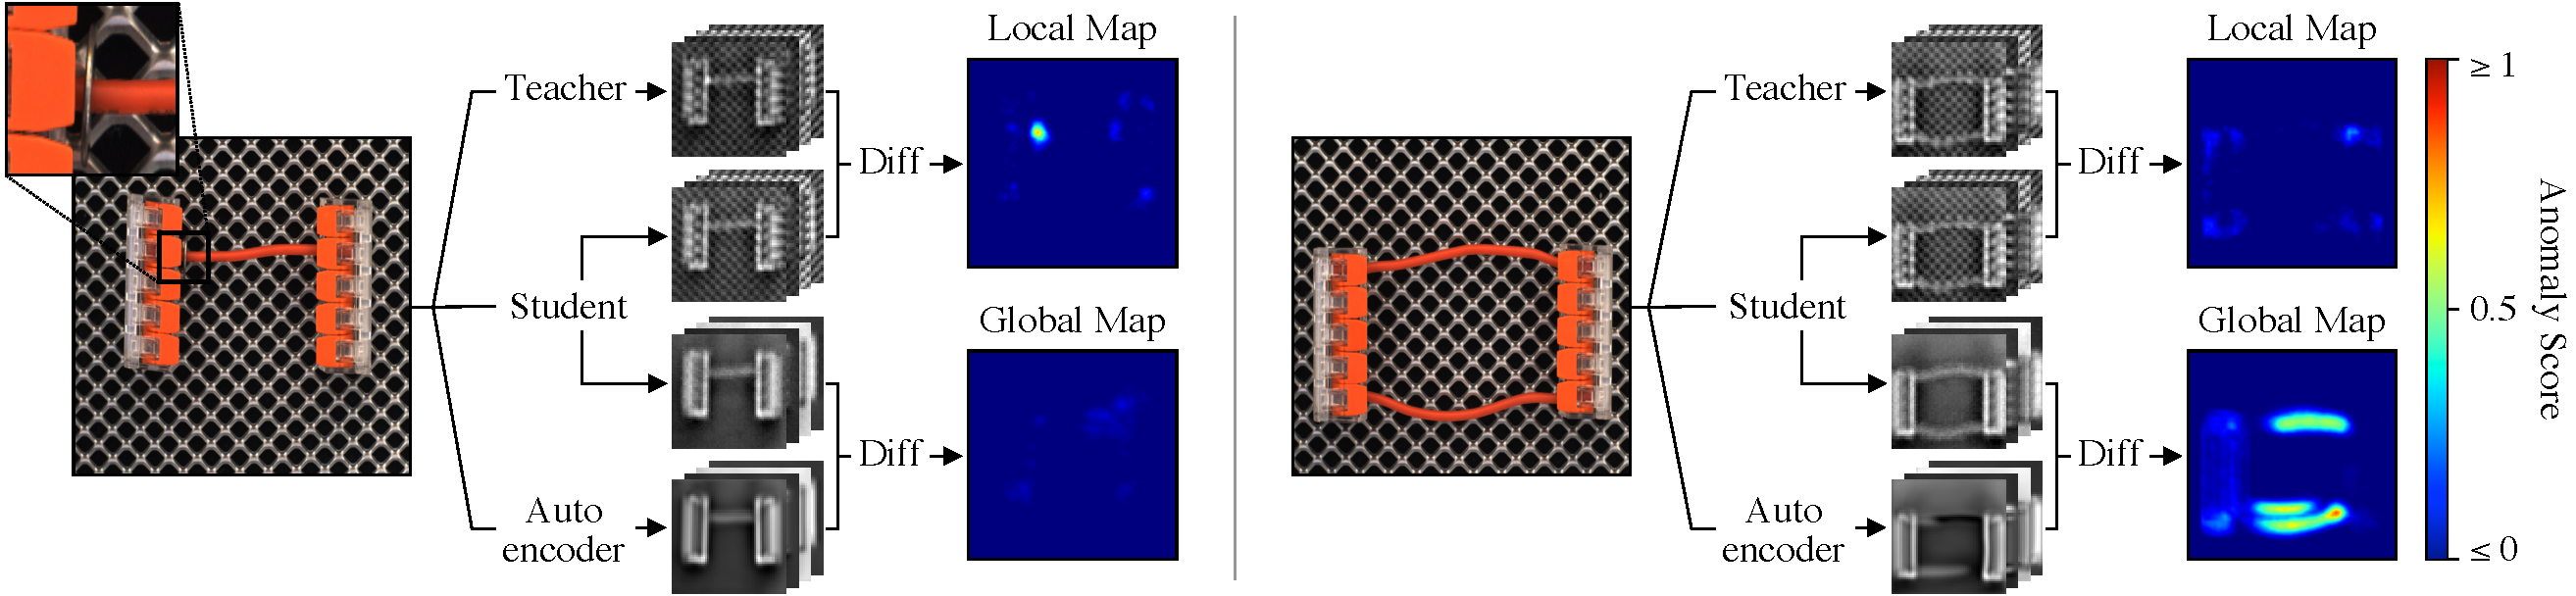
\includegraphics[width=1.1\linewidth]{Rohit_Master_Thesis/Images/efficientAD_pipeline.pdf}
    \caption{EfficientAD pipeline}
    \label{fig:EfficientAD pipeline}
\end{figure}

The student learns the systematic reconstruction errors of the autoencoder on normal images. However, it does not learn the reconstruction errors for anomalies as they are not part of the training set. This makes the difference between the student's and the autoencoder's output suitable for computing the anomaly map, which is calculated as the squared difference between the two outputs and then averaged across all channels. EfficientAD produces two anomaly maps, the one generated by the autoencoder-student pair is called a global anomaly map, and the one generated by \gls{s-t} pair is called a local anomaly map as seen in the figure \ref{fig:EfficientAD pipeline}. These two maps are then normalized to a similar scale and averaged to generate the combined anomaly map. Its maximum value is used as the image-level anomaly score \cite{batzner2024efficientadaccuratevisualanomaly}.

\subsubsection*{Performance :}

EfficientAD achieves an impressive image-level \gls{auroc} score of $99.8\%$ on MVTec AD dataset\cite{8954181} with early stopping enabled. For the overall anomaly detection performance, EfficientAD achieves very strong image-level detection and pixel-level localization performance with the highest score of $98.1$ for VisA\cite{zou2022spotthedifferenceselfsupervisedpretraininganomaly} dataset. The computational cost of EfficientAD was measured using the metrics latency and throughput, with the EfficientAD showing latency of $2.2ms$ and throughput of 614 $img/s$ \cite{batzner2024efficientadaccuratevisualanomaly}.

\subsection*{Summary of all the models}

The table \ref{tab:model_key_characteristics} summarizes all the models we have gone through above.

\begin{table}[ht!]
\centering
\resizebox{\textwidth}{!}{%
\begin{tabular}{|l|p{0.7\textwidth}|}
\hline
\textbf{Model} & \textbf{Key Characteristics} \\ \hline
YOLO & Real-time object detection; maps pixels to bounding box coordinates and class probabilities \\ \hline
PatchCore & Uses locally-aware patch features and memory banks for anomaly detection \\ \hline
DFM (Deep Feature Modelling) & Models normal data distribution using deep feature extraction and density modeling \\ \hline
EfficientAD & Combines lightweight student-teacher networks with efficient patch descriptors \\ \hline
FastFlow & Extends normalizing flow models to 2D for feature distribution estimation \\ \hline
DFKDE (Deep Feature Kernel Density Estimation) & Extracts features with \gls{dnn} and applies Kernel Density Estimation on reduced features \\ \hline
\end{tabular}%
}
\caption{Summary of Models and their Key Characteristics}
\label{tab:model_key_characteristics}
\end{table}

   % (\chapter{})
\clearpage
\chapter{Methods}

This section outlines the experimental procedures and processes carried out to conduct the research study. It includes datasets, the process of training \& testing the model, and metrics used to evaluate the method's performance.

\section{Dataset}
The dataset provided by Siemens consists of images of Solder joints on a \gls{pcb}. It has a total of 6014 images, each of $512 \times $512 dimensions, divided into \gls{fc} and \gls{ng}. The \gls{fc} class contains images without defects, while the \gls{ng} class contains images with various defects. The images are of two types, one is a colored image, as shown on the left of figures \ref{fig:dataset-NG} \& \ref{fig:dataset-FC}, and the other is a heat image, which is the red one on the right of the figures \ref{fig:dataset-NG} \& \ref{fig:dataset-FC}. This variation of images makes it suitable for evaluating various images for which a model can be used. The dataset is split into training and testing sets using an 80-20 split. A separate set of 160 images is also reserved for testing, finding accuracy, and visualizing classification and segmentation results.

\begin{figure}[ht!]
    \centering  
    \begin{minipage}{0.32\textwidth}
        \centering
        \includegraphics[width=\textwidth]{Images/Val_NG_BF2003043437_151_7_816_816_Color_origin.jpg} % Add your image file name here
        %\caption{An example of a defective piece of leather.}
    \end{minipage}
    \begin{minipage}{0.32\textwidth}
        \centering
        \includegraphics[width=\textwidth]{Images/Val_NG_BF2003033542_223_32_471_471_Multi_origin.jpg} % Add your image file name here
        %\caption{An example of a defective grid.}
    \end{minipage}\hfill
    \caption{Examples of defective solder joints in the dataset.}
    \label{fig:dataset-NG}
\end{figure}

\begin{figure}[ht!]
    \centering
    \begin{minipage}{0.32\textwidth}
        \centering
        \includegraphics[width=\textwidth]{Images/train_FC_BF2003015014_1174_42_2038_2038_Color.jpg} % Add your image file name here
        %\caption{An example of a defective piece of leather.}
    \end{minipage}
    \begin{minipage}{0.32\textwidth}
        \centering
        \includegraphics[width=\textwidth]{Images/Val_FC_heat_BF2003054784_4796_144_2042_2042_Multi.jpg} % Add your image file name here
        %\caption{An example of a defective tile.}
    \end{minipage}\hfill
    \caption{Examples of defect-free solder joints in the dataset.}
    \label{fig:dataset-FC}
\end{figure}

As can be seen in figure \ref{fig:dataset-NG} and figure \ref{fig:dataset-FC}, finding a defect without expertise can be challenging and time-consuming.

The table~\ref{tab:dataset-distribution} provides a detailed breakdown of the dataset distribution across subsets:

\begin{table}[ht!]
    \centering
    \begin{tabular}{|l|c|c|c|}
        \hline
        \textbf{Dataset} & \textbf{FC (No Defects)} & \textbf{NG (Defective)} & \textbf{Total} \\
        \hline
        Training & 2,971 & 1,712 & 4,683 \\
        \hline
        Testing & 743 & 428 & 1,171 \\
        \hline
        Custom Test & 80 & 80 & 160 \\
        \hline
    \end{tabular}
    \caption{Distribution of Images in the Dataset}
    \label{tab:dataset-distribution}
\end{table}

\section{Experiment}

Experiments were carried out using models mentioned in the section \ref{sec:unsupervised image processing}. All the models belong to Anomaly detection and are part of a deep learning library which has a collection of state-of-the-art anomaly detection algorithms called Anomalib. There are multiple steps taken in this experiment and they will be explained below.

\subsection{Data Loading}

To load and preprocess our dataset, we use Anomalib dataloader by importing \textbf{Folder} from \textbf{Data} class, specifically designed for handling our custom dataset, allowing for efficient data management and preprocessing. We create a Folder datamodule and configure several parameters as described below.

\textbf{Name :} It is the dataset configuration identifier, reflecting the specific dataset used for the experiment.

\textbf{Root Directory :} It points to the directory containing the organized dataset folders.

\textbf{Normal \& Abnormal Directories :} Models mostly require anomalous free images for training, which in our case is \gls{fc}, and anomalous images for testing(not used while training), which is \gls{ng}. So those are provided in these two fields.

\textbf{Normal Split Ratio :} The datamodule employs a 0.2 split ratio for validating normal images, which ensures a sufficient number of samples for model tuning and validation.

\textbf{Image Size :} All images are resized to $256 \times 256$ pixels during preprocessing, balancing the need for detailed feature representation with computational efficiency.

\textbf{Batch Size :} Both training and evaluation processes use different batch sizes for different models to optimize \gls{gpu} memory usage while maintaining effective gradient updates.

\textbf{Task Type :} There are two types of tasks available: classification and segmentation. For this thesis, for all the models, we have set the parameter to "CLASSIFICATION" and it directs the model to perform binary classification between the \gls{fc} and \gls{ng} categories.

\textbf{Number of Workers :} Based on the \gls{gpu} and the model being used, the number of workers varied between 0 to 8 for helping the computational resources to parallelize data loading.

%Model loading is carried out by importing. Here, each model is configured with a specific backbone, which serves as a feature extraction component. 

\subsection{Model Training or Inferencing}
\label{subsec:Model Training}

The training takes place in two steps here: first is loading the model, and second is the training part, which is explained below.

\textbf{Model Loading :} Firstly, the model of our choice is imported. The models used in this thesis are explained in \ref{sec:unsupervised image processing}. Each model is initialized with a specific backbone, such as '\gls{resnet}18', '\gls{resnet}50', 'Wide\gls{resnet}50' etc. These backbones are critical for feature extraction. The selection of the backbone and the specific layers used for feature extraction are the key factors that influence the model's ability to detect anomalies.

\textbf{Model Training or Inferencing :} Once the model is loaded, the next steps involve training or inferencing using the \textbf{Engine} class from Anomalib. Depending on the model we need to either train the model or just perform inferencing(extracting the features). The engine is configured to manage the complete process, ensuring that the model is trained effectively and can accurately infer from the data provided.

The key components of training/inferencing configuration are:

\textbf{Thresholding :} A threshold value determines the anomalous label for the calculated anomaly scores. There are two types of thresholding methods available; one is '\textbf{ManualThreshold}' where we have to set our own threshold value; this is beneficial in situations where there is a lack of appropriate representative validation data\cite{9897283}. The second one we have used is '\textbf{F1AdaptiveThreshold}'. The algorithm optimizes the value of the threshold to determine the optimal f1\_score and saves the calculated value of the adaptive threshold.\cite{Anomalib2024}

\textbf{Task Type :} The task is usually set to '\textbf{CLASSIFICATION}', which directs the model to categorize images into predefined classes (ex., normal and anomalous). Depending on the requirements, the task can also be configured to '\textbf{SEGMENTATION}' to pinpoint where the defect is there in the image.

\textbf{Image Metrics :} The model's performance is evaluated by '\textbf{\gls{auroc}}' and '\textbf{F1Score}'. These are standard metrics used for assessing classification accuracy and balance between precision and recall. These metrics are explained in section \ref{subsec:Evaluation Metrics}.

\textbf{Accelerator :} Depending on the available resources, the engine can run on a \textbf{'\gls{gpu}'}, \textbf{'\gls{cpu}'}, \textbf{'\gls{tpu}'}, \textbf{'\gls{ipu}'}, also there is an \textbf{'auto'} which chooses the appropriate resource automatically based on the availability.

\textbf{Devices :} This configuration allows us to provide the engine with the available number of devices(ex., \glspl{cpu}, \glspl{gpu}) to use during training and inference. The \textbf{'auto'} option sets the optimal devices automatically for the engine.

\textbf{Validation Frequency :} After every epoch \textbf{'check\_val\_every\_n\_epoch=1'}, this option validates the model, ensuring that the performance metrics are tracked throughout the training process.

\textbf{Max Epochs :} Depending on the model we are using, it can either required to be trained or do inferencing on. When the model performs inferencing at that time, the \textbf{'max\_epochs'} parameter is always set to \textbf{1}. Moreover, the models requiring training can be adjusted depending on the complexity of the model.%might need to add more info.

\textbf{Validation Check Interval :} The parameter \textbf{'val\_check\_interval'} sets when the validation checks are performed, in our case, it's set to \textbf{1.0}, meaning the validation checks are performed after every epoch.

After providing these training configurations to the engine class, we can call the \textbf{fit} function to start with the training or inferencing. Here, we provide the model and the datamodule components. Here, the \textbf{Normal} directory is used, which is the anomaly free images. After the training/inferencing is finished, the next step is to perform testing, which is explained in the section below.

\subsection{Testing}

After the training/inferencing is finished, we can move to the next critical step, i.e., to evaluate the model's performance. For this, the \textbf{test} function from the engine class is used, and similar to the fit function, we again need to pass the model and the datamodule components. Here, the \textbf{Abnormal} directory is used, which has the anomalous images. 

After the testing, its results are displayed, with two metrics mentioned in section \ref{subsec:Evaluation Metrics} \gls{auroc} and F1-Score.

\subsection{Model Exporting}
\label{subsec:Model Exporting}

Exporting a trained model is a very important task, as the model can then be deployed in real-world applications. This process involves converting the trained model into a format optimized for efficient inference on various hardware, like \glspl{cpu}, \glspl{gpu} etc. Thus, the model can be incorporated into production environments, operating at scale by processing new data and identifying anomalies in real time.

The Anomalib library lets us convert the models into formats like OpenVINO, ONNX, etc. We export our models into OpenVINO format. OpenVINO is an open-source software toolkit used to optimize and deploy \gls{dl} models. It minimizes resource requirements and effectively deploys on various platforms like the cloud. OpenVINO\textsuperscript{TM} enables inference on several hardware platforms, including \glspl{cpu}, \glspl{gpu}.\cite{openvino2024}

The export process is initialized by setting the desired export format via the \textbf{'ExportType'} variable. The trained model and the destination where the model should be exported are then passed to the \textbf{'Export'} function present in the engine class, which is responsible for the conversion. In the specified export location, three files are saved there:

\textbf{1. 'metadata.json'}, which stores the threshold value as mentioned in the section \ref{subsec:Model Training} based on which the classification can be done.

\textbf{2. 'model.bin'} is a binary file that contains the weights and biases of the model.

\textbf{3. 'model.xml'} this file stores the model's architecture. It contains the neural network structure, including layers, the connections between them, etc.

\section{Inference}
\label{subsec:Inference}

In the inference phase, the model is utilized to make predictions on new and unseen data. This section documents the approaches for achieving inference using a trained model, mainly focusing on two tasks: \textbf{'Image Classification'} and \textbf{'Image Segmentation'}. Both tasks are crucial in assessing the effectiveness of the model in detecting and localizing anomalies in solder joints on \glspl{pcb}.

Firstly, the trained model is loaded using the \textbf{'OpenVINOInferencer'} or \textbf{'TorchInferencer'} class, which can enable efficient inference on \glspl{cpu} or \glspl{gpu} respectively. Here, we will be using OpenVINOInferencer by providing the model and metadata paths of the trained model as explained in the section \ref{subsec:Model Exporting}. Once we are done creating the \textbf{'Inferencer'} object, we can move on to performing image classification and segmentation as described below.

\subsection{Image Classification}
\label{subsec:Image Classification}

Image Classification is an important task within \gls{cv} because it helps identify and recognize the object present in an image. It involves labeling input images based on their likelihood of being anomalous or not \cite{FANG2020100980}.

As mentioned in section \ref{subsec:Inference}, after creating the inference object then, we pass the input image to its \textbf{'predict'} function, which calculates the predicted label and the anomalous score. The predicted results are then visualized using \textbf{'ImageVisualizer'} class, which is configured for \textbf{CLASSIFICATION} mode, so it overlays the classification results on the input image, making it simpler to analyze the results.

\begin{figure}[ht!]
    \centering
    \includegraphics[width=1\linewidth]{Images/anomalous_image_classification.jpg}
    \caption{Image Classification on NG image}
    \label{fig:Image classification on NG image}
\end{figure}

Figure \ref{fig:Image classification on NG image} shows the result of image classification, where it gives three images as an output: first one is the input image, the second one shows the predicted heat map, which shows where the possible anomaly is and the third gives the prediction label and the score.

\subsection{Image Segmentation}
%\subsubsection{Metrics Calculation}

Image segmentation is a method of analyzing images at the pixel level. It involves utilizing multiple techniques to label each pixel as part of a particular class or instance\cite{IBM2024}. So, using image segmentation, we can point where the model has predicted the anomaly to be as shown in the figure \ref{fig:Image Segmentation on NG image}.

\begin{figure}[H]
    \centering
    \includegraphics[width=1\linewidth]{Images/anomalous_image_segmentation.jpg}
    \caption{Image Segmentation on NG image}
    \label{fig:Image Segmentation on NG image}
\end{figure}

\section{Evaluation Metrics}
\label{subsec:Evaluation Metrics}

Evaluation metrics play a crucial role in determining how well the \gls{ml} models have performed. These metrics aid in quantifying the model's ability to differentiate between anomalous and normal images, offering valuable insights into the model's effectiveness and areas for improvement. This section outlines the primary evaluation metrics used in this thesis: \gls{auroc}, Accuracy, Recall, Precision, F1-Score, and Confusion Matrix.

\subsection*{Area Under the Receiver-Operating Curve (AUROC)}
\label{subsec:AUROC}

The \gls{auroc} measures the ability of a classification model to differentiate across different classes. It has been particularly useful in measuring trade-offs of the \gls{tpr} (sensitivity) versus the \gls{fpr} (1-specificity) across different threshold settings. A higher \gls{auroc} value indicates better model performance, with a value of 1 representing a perfect model and a value of 0.5 indicating that the model that performs no better than random chance\cite{FAWCETT2006861}. This is extremely important for quality control applications because missing an anomaly can have severe consequences for a manufacturing process. %Write how its calculated in anomalib if possible

\subsection*{Accuracy}
\label{subsec:Accuracy}

Accuracy is the rate of correct predictions made by the model. It is often assessed using an unseen dataset that was never utilized throughout the learning process\cite{Kohavi1998}, like the custom test set mentioned in the table \ref{tab:dataset-distribution}. It is expressed as: 

\begin{equation}
    \text{Accuracy} = \frac{\text{\gls{tp}} + \text{\gls{tn}}}{\text{\gls{tp}} + \text{\gls{tn}} + \text{\gls{fp}} + \text{\gls{fn}}} \quad \text{\cite{Walker2024}}
    \label{eq:accuracy}
\end{equation}

Where \gls{tp}, \gls{tn}, \gls{fp}, and \gls{fn} are True Positives, True Negatives, False Positives, and False Negatives, respectively. It gives an overall view of the performance of the model.

\subsection*{Recall}
\label{subsec:Recall}

Recall, also known as sensitivity, refers to the ratio of accurately predicted positive cases to the total number of actual positive cases \cite{powers2020evaluationprecisionrecallfmeasure}. It is expressed as:

\begin{equation}
    \text{Recall} = \frac{\text{\gls{tp}}}{\gls{tp} + \gls{fn}} \quad \text{\cite{powers2020evaluationprecisionrecallfmeasure}}
    \label{eq:recall}
\end{equation}

A higher Recall value means that the model is good at detecting most anomalies, but it does not consider the number of \gls{fp}.

\subsection*{Precision}
\label{subsec:Precision}

Precision, also known as confidence, refers to the proportion of accurately predicted positive cases that are actually correct \cite{powers2020evaluationprecisionrecallfmeasure}. It is expressed as:

\begin{equation}
    \text{Precision} = \frac{\text{\gls{tp}}}{\gls{tp} + \gls{fp}} \quad \text{\cite{powers2020evaluationprecisionrecallfmeasure}}
    \label{eq:precision}
\end{equation}

This metric is very important where the cost of false positives is high, as it indicates how well the model can prevent the incorrect labeling of normal cases as anomalies. 

\subsection*{F1-Score}
\label{subsec:F1-Score}

The F1-score is a metric that achieves a balance between precision and recall. The calculation involves taking the harmonic mean of precision and recall. The F1-score is a valuable metric for achieving a trade-off between high precision and recall. It effectively penalizes extreme negative values of either component \cite{Walker2024}. It is expressed as:

\begin{equation}
\text{F1-Score} = 2 \times \frac{\text{Precision} \times \text{Recall}}{\text{Precision} + \text{Recall}} \quad \text{\cite{Walker2024}}
\end{equation}

It makes this metric valuable since it evaluates a models capability to detect anomalies(Recall) and its precision in identifying true positives without an excessive number of false positives. 

\subsection*{Confusion Matrix}
\label{subsec:Confusion Matrix}

A confusion matrix simply shows the predicted and actual classifications made by the model \cite{Kohavi1998}. It is a table containing the \gls{tp}, \gls{tn}, \gls{fp}, and \gls{fn} values. Subsequently, a Confusion Matrix can help explain the errors a model makes so that improvements can be made specifically within the same area.

\begin{figure}[ht!]
    \centering
    \includegraphics[width=1\linewidth]{Images/confusion matrix.png}
    \caption{Example of Confusion Matrix}
    \label{fig:confusion matrix}
\end{figure}

Figure \ref{fig:confusion matrix} shows a confusion matrix from one of our models. Here, the \gls{tp} is the top-left corner dark blue cell, \gls{tn} is the bottom-right dark blue cell, \gls{fp} is the bottom-left light blue cell, and \gls{fn} is the upper-right light blue cell.



\clearpage
\chapter{Results}

This section presents the detailed findings and results of our experiments using various unsupervised anomaly detection models for the task of identifying faulty solder joints in \gls{pcb}. The models which we have evaluated here are PatchCore(section \ref{subsec:patchcore}), \gls{dfm}(section \ref{subsec:dfm}), \gls{dfkde}(section \ref{subsec:dfkde}), EfficientAD(section \ref{subsec:efficientad}), FastFlow(section \ref{subsec:fastflow}), which uses different hyperparameters, feature extraction backbones and its layers. We aim to study the effectiveness of these models in comparison to the current baseline models used by Siemens \gls{yolo}(section \ref{subsec:yolo}) while also the factors affecting their performances.

\section{Overall Performance of Models}

The table \ref{tab:overall model accuracy} and the bar chart \ref{fig:bar chart models accruacy} represent each model's overall accuracy performance, giving an initial overview of how these models compare in terms of how they classify anomalies correctly.

\begin{table}[ht!]
    \centering
    \begin{tabular}{|l|l|}
        \hline
        \textbf{Model} & \textbf{Accuracy} \\ \hline
        \textbf{Yolov8-L} & \textbf{95\%} \\ \hline
        \textbf{Yolov8-M} & \textbf{93.75\%} \\ \hline
        \textbf{PatchCore} & \textbf{91.25\%} \\ \hline
        Deep Feature Modeling(DFM) & 72.85\% \\ \hline
        Deep Feature Kernel Density Estimation(DFKDE) & 70.71\% \\ \hline
        FastFlow & 66.87\% \\ \hline
        EfficientAD & 60\% \\ \hline
    \end{tabular}
    \caption{Overall comparison of different models accuracy}
    \label{tab:overall model accuracy}
\end{table}

The chart \ref{fig:bar chart models accruacy} provides a graphical representation of the same data of each model's accuracy, where we can clearly visualize the performance of different models. As can be seen in table \ref{tab:overall model accuracy} and bar chart \ref{fig:bar chart models accruacy} the baseline model \gls{yolo}v8-L achieves the highest accuracy of 95\%, while \textbf{the best performing unsupervised model is PatchCore closely following with an accuracy of 91.25\%, with only a 2.5\% difference in the accuracy of baseline model \gls{yolo}v8-M}. Other models, such as \gls{dfm}, \gls{dfkde}, FastFlow, and EfficientAD, show moderate performance. Here, none of the unsupervised anomaly detection models could overtake the supervised baseline model. One of the reasons for this is that the baseline model was trained in a supervised fashion, where it had access to all the labels of the image dataset. Whereas the anomaly detection models were not given any labels for the images, and while training, only anomaly free data was used, it had to figure out on its own which images were anomalous and which images were normal.

\begin{figure}[ht!]
    \centering
    \includegraphics[width=1.1\linewidth]{Rohit_Master_Thesis//Images/bar_chart_model_acc.png}
    \caption{Bar chart representation of the different models accuracy like \gls{yolo}(baseline), our approach including PatchCore, \gls{dfm}, \gls{dfkde}, FastFlow, and EfficientAD.}
    \label{fig:bar chart models accruacy}
\end{figure}

\section{Model-wise breakdown of results}

\subsection*{PatchCore}

\begin{figure}[H]
    \centering
    \includegraphics[width=1\linewidth]{Rohit_Master_Thesis//Images/patchcore heatmap.png}
    \caption{PatchCore heatmap for the experiment where backbone "Wide Resnet50" and different layers were used.}
    \label{fig:patchcore heatmap}
\end{figure}

\iffalse
\begin{figure}[ht!]
    \centering  
    % First image
    \begin{minipage}{0.6\textwidth}
        \centering
        \includegraphics[width=\textwidth]{Rohit_Master_Thesis//Images/patchcore_config1_confusion_matrix.jpg} % Add your image file name here
        \caption{Configuration 1}
    \end{minipage}
    
    \vspace{0.5cm} % Adds vertical space between images
    
    % Second image
    \begin{minipage}{0.6\textwidth}
        \centering
        \includegraphics[width=\textwidth]{Rohit_Master_Thesis//Images/patchcore_config2_confusion_matrix.jpg} % Add your image file name here
        \caption{Configuration 2}
    \end{minipage}
    
    \vspace{0.5cm} % Adds vertical space between images
    
    % Third image
    \begin{minipage}{0.6\textwidth}
        \centering
        \includegraphics[width=\textwidth]{Rohit_Master_Thesis//Images/patchcore_config3_confusion_matrix.jpg} % Add your image file name here
        \caption{Configuration 3}
    \end{minipage}
    
    \caption{Comparison of Confusion Matrices for Different Configurations.}
    \label{fig:dataset-NG}
\end{figure}
\fi

For this experiment, we employed PatchCore with \texttt{wide\_resnet50\_2} backbone as feature extraction for performing anomaly detection. Firstly, the model extracts feature representations from specific layers of the backbone and then compares the patch-level features of test images with those stored in a memory bank built from normal data. PatchCore uses \gls{k-nn} retrieval for detecting deviations from nominal behavior by calculating the anomaly score based on the distance between patches from the test image and their closest counterparts in the memory bank. This allows PatchCore to perform well when the labeled data is not abundantly available. This model is explained in more detail in \ref{subsec:patchcore}.

For the first configuration, we have used backbone \texttt{wide\_resnet50\_2} with layer2 and layer3 as shown in the heatmap \ref{fig:patchcore heatmap}. This configuration achieves an \gls{auroc} score of 0.8816 and an overall accuracy of 83.75\%. The F1-score was relatively strong at 0.8571, suggesting that the model maintained a balance between precision and recall. The model had a precision of 0.7647, suggesting that sometimes the model classified normal data as anomalous, which resulted in moderate occurrence of false positives, as can be confirmed by the confusion matrix \ref{fig:patchcore config1 confusion matrix}. Whereas the high recall value of 0.975 indicates that the model was highly accurate in detecting almost all the anomalies as anomalies, with some false negatives, as can be seen in the figure \ref{fig:patchcore config1 confusion matrix}.

\begin{figure}[ht!]
    \centering
    \includegraphics[width=1\linewidth]{Rohit_Master_Thesis//Images/patchcore_config1_confusion_matrix.jpg}
    \caption{Confusion matrix for the first configuration where backbone "Wide Resnet50" and layers "2, 3" were used.}
    \label{fig:patchcore config1 confusion matrix}
\end{figure}

The second configuration resulted in the best overall performance across all metrics, where the feature extraction was carried out by layer1 and layer2 of the same backbone \texttt{wide\_resnet50\_2}. This configuration resulted in a high \gls{auroc} score of 0.9271, with a significant increase in accuracy of 91.25\% as shown in the heatmap \ref{fig:patchcore heatmap}. We also saw improvement in F1-score by about 6.6\% from the previous configuration, reaching 0.9176, indicating an even better balance between precision and recall. The precision improved to 0.8667, indicating a reduction in false positives as seen in the confusion matrix \ref{fig:patchcore config2 confusion matrix} where the false positives were reduced by 50\% from the first configuration. While the recall remained high but the same as the first configuration at 0.975, meaning the model continued to detect almost all anomalies, as shown in the figure \ref{fig:patchcore config2 confusion matrix}. The improved performance of this configuration can be due to the use of features from the combination of layer 1 and layer 2, which incorporates the combination of both low-level and mid-level features. Low-level features might allow the model to detect fine-grained details, while layer 2 might provide the more complex structures needed to detect anomalies. These features can provide a richer, more detailed representation of normal data, making the detection of anomalies without overfitting normal data easier.

\begin{figure}[ht!]
    \centering
    \includegraphics[width=1\linewidth]{Rohit_Master_Thesis//Images/patchcore_config2_confusion_matrix.jpg}
    \caption{Confusion matrix for the second configuration where backbone "Wide Resnet50" and layers "1, 2" were used.}
    \label{fig:patchcore config2 confusion matrix}
\end{figure}

In the third configuration, layer 2, layer 3, and layer 4 were used for the backbone \texttt{wide\_resnet50\_2}, it resulted in a lower \gls{auroc}score of 0.8807 which is almost equal to the \gls{auroc} score for first configuration, and the accuracy we got is 76.25\% which is the lowest of all the configuration. The F1-score also decreased slightly to 0.8061 due to a drop in precision value to 0.6810. This lower precision indicates that the model produced a higher number of false positives, i.e., more normal images were classified as anomalous, as can be seen in confusion matrix \ref{fig:patchcore config3 confusion matrix} where out of 80 normal images, 37 were classified as anomalous. However, the recall was the highest at 0.9875, which means that the model was still able to detect almost all of the anomalies, as seen in the figure \ref{fig:patchcore config3 confusion matrix} out of 80, 79 were correctly classified as anomalous with only one being misclassified as normal. The inclusion of deeper layers, like layer 4, probably introduced more abstract features, which may have been less effective for the detection of fine-grained anomalies, resulting in the reduction of overall performance. This configuration highlights the importance of extraction of features from appropriate layers for ensuring balance between detecting true anomalies and avoiding excessive false positives.

\begin{figure}[ht!]
    \centering
    \includegraphics[width=1\linewidth]{Rohit_Master_Thesis//Images/patchcore_config3_confusion_matrix.jpg}
    \caption{Confusion matrix for the third configuration where backbone "Wide Resnet50" and layers "2, 3, 4" were used.}
    \label{fig:patchcore config3 confusion matrix}
\end{figure}

Now let's look at how the best performing configuration of PatchCore image classification results. When performing image classification

\begin{figure}[ht!]
    \centering  
    \begin{minipage}{1\textwidth}
        \centering
        \includegraphics[width=1\textwidth]{Rohit_Master_Thesis//Images/IC_NG.png} % Add your image file name here
        %\caption{Caption for the first image.}
    \end{minipage}
    
    %\vspace{5pt} % Adjust the space between images

    \begin{minipage}{1\textwidth}
        \centering
        \includegraphics[width=1\textwidth]{Rohit_Master_Thesis//Images/IC_FC.png} % Add your image file name here
        %\caption{Caption for the second image.}
    \end{minipage}
    
    %\vspace{10pt} % Adjust the space between images

    \begin{minipage}{1\textwidth}
        \centering
        \includegraphics[width=1\textwidth]{Rohit_Master_Thesis//Images/IC_NG2.png} % Add your image file name here
        %\caption{Caption for the third image.}
    \end{minipage}
    
    \caption{Results of image classification using second configuration.}
    \label{fig:dataset-NG-vertical}
\end{figure}


\subsection*{\gls{yolo}}

Two different model sizes of \gls{yolo}v8 \cite{Ultralytics2024} were evaluated for this experiment: \gls{yolo}v8-M(medium) and \gls{yolo}v8-L(large). Both the models were trained for 200 epochs on the training dataset.

The \textbf{\gls{yolo}v8-L} model, which is larger and more complex, reached an accuracy of 95\% after 200 epochs. The model's high accuracy could be due to its increase in the depth and number of parameters, which allows it to capture more detailed and complex patterns in the dataset. Also it being a supervised model, having access to all the labels while training helps it to learn better and fit the model well to the data.

\begin{figure}
    \centering
    \includegraphics[width=1.3\linewidth]{Rohit_Master_Thesis//Images/yolov8l_confusion_matrix.png}
    \caption{Confusion matrix for the baseline model \gls{yolo}v8-L, its accuracy is 95\%}
    \label{fig:yolov8l confusion matrix}
\end{figure}

The confusion matrix, as shown in figure \ref{fig:yolov8l confusion matrix}, provides a more detailed look into how well the model performs in the classification task. We can see that the model was able to correctly classify all the normal(FC) images as normal. While only 6 were false positives, i.e., anomalous(NG) images were classified as normal images, the rest of the 74 were correctly classified as NG, i.e., True Negatives. These values are consistent with the precision, recall, and F1-score results as shown in table \ref{tab:yolov8_performance}. The precision of 1.0 highlights the model's reliability in predicting normal(FC) instances, as it did not make any incorrect predictions for that class. The recall of 0.925, while still quite good, indicates that the model misclassified a small number of anomalous(NG) as normal(FC). With the impressive F1-score of 0.9615, shows the models well-rounded performance.

\begin{table}[ht!]
    \centering
    \begin{tabular}{|c|c|c|c|c|}
        \hline
        \textbf{Model} & \textbf{Accuracy} & \textbf{Precision} & \textbf{Recall} & \textbf{F1-score} \\ \hline
        \textbf{YOLOv8-M} & 93.75\% & 0.9867 & 0.925 & 0.9547 \\ \hline
        \textbf{YOLOv8-L} & 95\% & 1.0 & 0.925 & 0.9615 \\ \hline
    \end{tabular}
    \caption{Comparison of YOLOv8-M and YOLOv8-L Model Performance}
    \label{tab:yolov8_performance}
\end{table}

%Probably for discussion section(remember to paraphrase)
%Explanation of Results
%The performance of YOLOv8-L is in line with its design as a larger, more powerful model. The depth and complexity of the YOLOv8-L architecture allow it to capture a wide variety of patterns and features in the data, leading to its high precision and recall. The non-maximum suppression (NMS) technique used in YOLOv8 helps further refine the predictions by ensuring that overlapping bounding boxes are filtered, resulting in more accurate object classification. Additionally, YOLOv8-L's anchor-free detection mechanism improves its ability to generalize across objects of various sizes, contributing to its robustness in detecting NG and FC items.

The \textbf{\gls{yolo}v8-M} model, which is smaller and more lightweight when compared to \gls{yolo}v8-L, reaches an accuracy of 93.75\%. This is slightly lower than its bigger model, as seen from the table \ref{tab:yolov8_performance}, but its overall performance was still quite impressive.

\begin{figure}[ht!]
    \centering
    \includegraphics[width=1.3\linewidth]{Rohit_Master_Thesis//Images/yolov8m_confusion_matrix.png}
    \caption{Confusion matrix for the baseline model \gls{yolo}v8-M, its accuracy is 93.75\%}
    \label{fig:yolov8m confusion matrix}
\end{figure}

The confusion matrix in figure \ref{fig:yolov8m confusion matrix} shows almost similar results to that of \gls{yolo}v8-L. With 79 True positives and 74 true negatives, while only making 6 false positives and 1 false negative prediction, apart from the 1 misclassified normal image as anomalous, the results are similar to that of \gls{yolo}v8-L. This indicates that the performance of the \gls{yolo}v8-M, though highly accurate, still falls just short of \gls{yolo}v8-L's performance due to its smaller capacity for learning complex patterns. As can be seen from the table \ref{tab:yolov8_performance}, the model achieved a precision of 0.9867, meaning that almost all of the predictions of normal(FC) images were correct. The recall for both the \gls{yolo}v8-L and \gls{yolo}v8-M matches and is equal to 0.925, indicating that both models successfully detected the same number of FC cases. The F1-score of the model was 0.9547, which is slightly lower than \gls{yolo}v8-L due to the slight decrease in the precision. While the model was highly accurate, it did produce a small number of false positives, in this case, 6 anomalous(NG) images were misclassified as normal(FC), which reduced its precision slightly.

%See if you need to include loss and accuracy curve for both the models of YOLO

%Probably for discussion section(remember to paraphrase)
%Explanation of Results

%YOLOv8-M strikes a balance between computational efficiency and accuracy. The model achieves 93.75\% accuracy, which is competitive given its smaller architecture compared to YOLOv8-L. The slightly lower performance is expected due to YOLOv8-M’s reduced depth and number of parameters, which limits its ability to capture as many intricate patterns in the data as YOLOv8-L. However, YOLOv8-M’s simpler structure makes it faster and more computationally efficient, making it suitable for tasks where real-time performance and resource limitations are important.

%Model Comparison and Insights
%YOLOv8-L outperforms YOLOv8-M by achieving 95\% accuracy, compared to YOLOv8-M’s 93.75\%. This difference in performance can be attributed to the larger number of layers and parameters in YOLOv8-L, which allows it to capture more detailed features from the dataset. YOLOv8-L’s larger architecture is particularly beneficial for classification tasks that involve complex patterns or subtle differences between classes, making it a better choice for applications where accuracy is critical.

%However, YOLOv8-M offers significant advantages in terms of speed and computational efficiency. Despite having fewer layers, YOLOv8-M achieves strong results, making it a good option for scenarios where real-time inference is necessary or where computational resources are limited. The slight trade-off in accuracy is reasonable given the gains in efficiency, making YOLOv8-M ideal for environments where fast processing is prioritized over achieving the highest possible accuracy.

\subsection*{\gls{dfm}}

In this section, we will look into the results obtained from various experiments using \gls{dfm}. \gls{dfm} is explained in the section \ref{subsec:dfm}, and in our experiments, we evaluated \gls{dfm} performance using various backbones, their layers, and pooling techniques to explore the robustness and accuracy of the model. Below the results are divided based on the backbone used. 

\subsubsection*{ResNet50}

Here, we used ResNet50's layer4 for feature extraction along with \gls{nll} as the scoring type. This gave us the \gls{auroc} score of 0.6309 and F1-score of 0.6689, with an overall accuracy of 50.7\%, which is not very good, as can be seen from the table \ref{tab:dfm resnet results}, it is basically doing random guessing. The low F1-score suggests that while the model was good at detecting anomalies, it struggled with precision because of the high number of false positives. These findings suggest that using features extracted from higher layers, like layer 4, may have led the model to focus on more abstract, high-level features that are less effective at determining anomalies from normal samples.

\begin{table}[ht!]
    \centering
    \begin{tabular}{|l|c|c|c|c|c|}
        \hline
        \textbf{Model} & \textbf{Accuracy (\%)} & \textbf{\gls{auroc}} &\textbf{Precision} & \textbf{Recall} & \textbf{F1-score} \\ \hline
        ResNet50 & 50.71\% & 0.6309 & 0.5036 & 1.0 & 0.6699 \\ \hline
        Wide-ResNet50-2 (layer2, nll) & 60\% & 0.6382 & 0.5556 & 1.0 & 0.7143 \\ \hline
        Wide-ResNet50-2 (layer2, fre) & 62.12\% & 0.5795 & 0.5681 & 1.0 & 0.7254 \\ \hline
        Wide-ResNet50-2 (layer3) & 62.86\% & 0.7265 & 0.5738 & 1.0 & 0.7292 \\ \hline
    \end{tabular}
    \caption{Results for ResNet and Wide-ResNet50-2 Backbones}
    \label{tab:dfm resnet results}
\end{table}

Another configuration that we tried was using a different variant of ResNet50 called Wide-ResNet50-2 and performing feature extraction using layer 2 while keeping the \gls{pca} level at 0.97 and using \gls{nll} score type. This resulted in a slight improvement in both the accuracy and \gls{auroc} score of 60\% and 0.6382, respectively. The precision improved to 0.5556, while the recall stayed at 1.0, resulting in an F1-score of 0.7143, as shown in the table \ref{tab:dfm resnet results}. Along with that, we also performed a similar experiment by keeping the backbone and layer the same but changing the \gls{pca} level to 0.995 and scoring type to \gls{fre}. This resulted in much better compared to when we used scoring type as \gls{nll}, where accuracy increased by about 2\% to 62.12\% while seeing a drop in \gls{auroc} to 0.5795. The recall stayed the same at 1.0, but a slight increase in precision was observed to 0.5681, therefore increasing the F1-score to 0.7254. This improvement in both precision and F1-score shows that lower-level features from layer 2 were more effective at capturing variations between normal and anomalous images. Finally, after seeing better results with \gls{fre} scoring type, we experimented with one more layer of the same backbone. The layer used here was layer 3, and with this, we again saw slight improvement across all the metrics. The accuracy came out to be 62.86\% which is a small incremental update, while with \gls{auroc} score we saw an improvement of about 25\% when compared to Wide-ResNet50-2 (layer2, \gls{fre}) of the table \ref{tab:dfm resnet results}, and saw a rise of about 14\% when compared with Wide-ResNet50-2 (layer2, \gls{nll}). Other layers were also tried for both the ResNet50 and Wide-ResNet50-2 backbone, but all of them resulted in the model just randomly guessing the predictions, i.e., the accuracy was 50\%.

\subsubsection*{Densenet}

Next, we conducted experiments using different DenseNet backbones. Firstly, we used DenseNet121, which extracted features from the features.norm5 layer and the \gls{fre} score type. This configuration improved the model's performance further, with an \gls{auroc} score of 0.7309 and an accuracy of 61.43\%. The model reached a precision of 0.5645 and a recall of 1.0, giving an F1-score of 0.7216. These improved scores suggest that the DenseNet architecture, which relies on dense connections and feature reuse, contributed to improved feature representations for anomaly detection. Table \ref{tab:dfm densenet results} shows the results of different backbones of DenseNet.

\begin{table}[ht!]
    \centering
    \begin{tabular}{|l|c|c|c|c|c|}
        \hline
        \textbf{Model} & \textbf{AUROC} & \textbf{Accuracy} & \textbf{Precision} & \textbf{Recall} & \textbf{F1-score} \\ \hline
        DenseNet121 & 0.7310 & 0.6143 & 0.5645 & 1.0 & 0.7216 \\ \hline
        DenseNet169 (norm5) & 0.7456 & 0.6571 & 0.5932 & 1.0 & 0.7447 \\ \hline
        \textbf{DenseNet169 (denseblock3, 0.97 PCA)} & \textbf{0.7203} & \textbf{0.7286} & 0.6538 & 0.9714 & 0.7816 \\ \hline
        DenseNet169 (denseblock3, 0.995 PCA) & 0.7190 & 0.7214 & 0.6422 & 1.0 & 0.7821 \\ \hline
        DenseNet201 (denseblock3, 0.995 PCA) & 0.7259 & 0.7143 & 0.6389 & 0.9857 & 0.7753 \\ \hline
        %DenseNet264d (untrained) & 0.8029 & N/A & N/A & N/A & 0.8471 \\ \hline
        %DenseNet201 (denseblock3, 0.97 PCA) & 0.7265 & N/A & N/A & N/A & 0.8460 \\ \hline
    \end{tabular}
    \caption{Results for DenseNet Backbones}
    \label{tab:dfm densenet results}
\end{table}

The best performing configuration for the DenseNet architecture comes from the DenseNet169 backbone, with features extracted from features.denseblock3 layer, a \gls{pca} level of 0.97, and the \gls{fre} score type as shown in the table \ref{tab:dfm densenet results}. This configuration gave an \gls{auroc} score of 0.7203 and an accuracy of 72.86\%. Precision also improved to 0.6538. While recall reduced slightly, it remained high at 0.9714, resulting in an F1-score of 0.7816. This improvement in both the precision and the F1-score suggests that the DenseNet169's larger size allowed for better feature extraction and classification, particularly when extracting features from the third dense block. The high recall score indicates that the model was able to detect most of the anomalies, as can be seen in the confusion matrix \ref{fig:dfm densenet169 confusion matrix}, while the increase in precision value indicates a significant reduction in the number of false positives relative to other configurations.

\begin{figure}[ht!]
    \centering
    \includegraphics[width=1\linewidth]{Rohit_Master_Thesis//Images/dfm_densenet_best_confusion_matrix.png}
    \caption{Confusion matrix for the best performing configuration for \gls{dfm} model with DenseNet169 backbone, its accuracy is 72.86\%}
    \label{fig:dfm densenet169 confusion matrix}
\end{figure}

After getting good results with the configuration explained above, we thought of checking another variation of the DenseNet169 backbone while keeping the feature extraction layer and scoring type the same as before but using a higher \gls{pca} level of 0.995, allowing for a greater variance in the data. However, the results were more or less similar to the previous configuration, with a slightly lower \gls{auroc} of 0.7190 and an accuracy of 72.14\%, along with a precision of 0.6422 and an F1-score of 0.7821. The recall remained at 1.0, but the decrease in precision compared to the previous configuration indicates that the increased retained variance caused the model to classify a higher number of normal images as anomalous. Finally, DenseNet201 was also tested with the same feature extraction layer, keeping the other hyperparameters the same. This configuration also gave similar results to previous ones highlighted in the table \ref{tab:dfm densenet results}.


% In discussions explain also the difference between scoring type fre and nll
% In discussion also discuss why was the recall for most part 1.0

\subsection*{\gls{dfkde}}

Here, we discuss the results obtained for the model \gls{dfkde}. It combines the power of \gls{dl} with statistical methods like \gls{pca} and \gls{kde}. The model first extracts robust features using a pre-trained deep neural network, then reduces their dimensionality by using \gls{pca}, and finally applying \gls{kde} to model the distribution of normal data. Two backbones were tested in this experiment, namely ResNet18 and Wide-ResNet50. The overview of the results for different configurations in the form of a bar chart is shown in figure \ref{fig:dfkde model results}.

\begin{figure}[ht!]
    \centering
    \includegraphics[width=1.2\linewidth]{Rohit_Master_Thesis//Images/dfkde_model_results.png}
    \caption{DFKDE model results for different backbones. The values shown here include \gls{auroc} score, F1-score, accuracy, and precision.}
    \label{fig:dfkde model results}
\end{figure}

\subsubsection*{ResNet18}

For the first experiment with the ResNet18 backbone, we use the feature extraction layer 1. This configuration aims at capturing the lower-level basic features and is trained with a maximum of 3000 training points to fit the \gls{kde} model.

Its results are shown in the table \ref{tab:dfkde resnet18 results}. As can be seen, the performance is not quite good, with \gls{auroc} score of 0.7364 and an accuracy of 57.86\%. Precision is quite low at 0.5447, while recall is high at 0.9571, resulting in an F1-score of 0.6943. The lower precision value indicates that the features extracted from the lower layer lead to the introduction of noise, leading to higher false positives. While the high recall value suggests that the model was still able to detect most of the anomalies correctly. However, the overall performance of the model still suffered as low-level features are less effective in anomaly detection for \gls{dfkde} model.

\begin{table}[ht!]
    \centering
    \begin{tabular}{|l|c|c|c|c|c|c|}
        \hline
        \textbf{Configuration} & \textbf{AUROC} & \textbf{Accuracy(\%)} & \textbf{Precision} & \textbf{Recall} & \textbf{F1-Score} \\ \hline
        Layer1, max training points 3000 & 0.7364 & 57.86\% & 0.5447 & 0.9571 & 0.6943 \\ \hline
        Layer2, max training points 3000 & 0.7535 & 65.71\% & 0.6078 & 0.8857 & 0.7209 \\ \hline
        Layer3, max training points 3000 & 0.7428 & 70.71\% & 0.6355 & 0.9714 & 0.7684 \\ \hline
        Layer3, max training points 5000 & 0.7310 & 68.57\% & 0.6182 & 0.9714 & 0.7556 \\ \hline
    \end{tabular}
    \caption{Results for DFKDE Model with ResNet18 Backbone}
    \label{tab:dfkde resnet18 results}
\end{table}

For the second experiment with the ResNet18 backbone, we used feature extraction layer 2, and the number of maximum data points for \gls{kde} model remained the same as before at 3000.

The model achieved an \gls{auroc} score of 0.7535, which is slightly better than when features were extracted from layer 1, an accuracy of 65,71\% is observed, which is about 14\% higher than that of configuration 1, as can be seen in the table \ref{tab:dfkde resnet18 results}. A precision of 0.6078 and a recall of 0.8857, resulting in an F1-score of 0.7209. This improvement in \gls{auroc} score and precision indicates that the mid-level features are more effective in anomaly detection for \gls{dfkde} model as they maintain the balance of the low-level details and high-level semantic information. Even though recall is slightly reduced compared to layer 1, the improvement in precision indicates a reduction in false positives.

For the third experiment, we select layer 3 for feature extraction of the backbone ResNet18, which is responsible for capturing higher-level semantic information. This layer offers a more abstract representation of the input data, which can be particularly suitable for anomaly detection tasks. This configuration was the best performing one in the \gls{dfkde} model.

As shown in the table \ref{tab:dfkde resnet18 results} an \gls{auroc} score of 0.7427, an accuracy of 70.71\% which is more than 22\% higher than configuration 1, and more than 7\% higher than configuration 2. A further improvement in precision was observed at 0.6355, and a recall of 0.9714, leading to an F1-score of 0.7684. The layer 3 features give more abstract representations of the data, which helped reduce false positive rates further while also maintaining high recall. However, a slight dip in \gls{auroc} compared to layer2 configuration can indicate that while the high-level features are useful, they might lack some of the finer details necessary for achieving good anomaly detection performance.

Next, for the fourth experiment, to examine the effects of increasing the number of training points, we increased the max training points parameter to 5000 points to fit the \gls{kde} model while keeping the backbone and the feature extraction layer the same as ResNet18 layer3. The goal was to see if more training data would improve \gls{kde}'s ability to model normal distribution, as layer 3 gave the best results.

In table \ref{tab:dfkde resnet18 results}, we can see that the model reached an \gls{auroc} score of 0.7310, with an accuracy of 68.57\%, which is lower than the third experiment, and with precision and recall of 0.6182 and 0.9714 respectively, leading to an F1-score of 0.7556. The performance was slightly worse than that of configuration 3, where layer 3 with 3000 max training points was used. This indicates that the number of training points may be less important than the layer from which the features are extracted, at least beyond a threshold.

\subsubsection*{Wide-ResNet50}

The second backbone we experimented with was Wide-ResNet50-2, which is a wider version of the standard ResNet50 architecture. In this experiment, features were extracted using layer 2 of the backbone. This configuration was chosen because the middle layer performed better for the ResNet18 backbone experiments and with the wider architecture, which can capture more detailed feature representations, which could possibly improve the anomaly detection performance.

\begin{table}[ht!]
    \centering
    \begin{tabular}{|l|c|c|c|c|c|c|}
        \hline
        \textbf{Configuration} & \textbf{AUROC} & \textbf{Accuracy(\%)} & \textbf{Precision} & \textbf{Recall} & \textbf{F1-Score} \\ \hline
        Layer2, max training points 3000 & 0.7725 & 67.86\% & 0.6344 & 0.8429 & 0.7239 \\ \hline
    \end{tabular}
    \caption{Results for DFKDE Model with Wide-ResNet50-2 Backbone}
    \label{tab:dfkde wide-resnet50 results}
\end{table}


This configuration showed improved performance in \gls{auroc} score and precision as seen from the table \ref{tab:dfkde wide-resnet50 results} of 0.7725 and 0.6344, respectively. The accuracy was 67.86\%, and the recall fell to 0.8429, resulting in the F1-score of 0.7239. The wider architecture and mid-level features from layer 2 did help the model capture more subtle patterns in the data, which resulted in a higher \gls{auroc} score when compared to ResNet18 experiments. The precision also slightly improved, indicating that the model was comparatively more accurate in detecting true anomalies. However, the lowest recall value of all the experiments combined from resNet18 and Wide-ResNet50 indicates that the model became slightly less sensitive to anomalies, likely as a result of the increase in specificity brought by the wider backbone.

\subsection*{FastFlow}

For this experiment, we used the FastFlow model with ResNet18, Wide-ResNet50-2, \gls{deit}, \gls{cait} as backbones for feature extraction. An overview of all the results is shown in the form of a bar chart in the figure \ref{fig:fastflow model results}. The best performing configuration in terms of accuracy was the one where \gls{deit} architecture was used for feature extraction, achieving 66.87\%. Below, we will discuss all the experiments and their results in detail, grouped based on the backbones used. Here, all the models were trained for 50 epochs except for when callback functionality was used. Then, it is trained until a condition is met.

\begin{figure}[H]
    \centering
    \includegraphics[width=1.2\linewidth]{Rohit_Master_Thesis//Images/fastflow_model_results.png}
    \caption{FastFlow model's results bar-chart for different configurations and backbones used for feature extraction.}
    \label{fig:fastflow model results}
\end{figure}

\subsubsection*{ResNet18}

For the first experiment, we have used ResNet18 as the backbone for feature extraction. This configuration achieved an \gls{auroc} score of 0.9199, which is quite good, and it demonstrates the models effectiveness in distinguishing normal images from abnormal ones on training and testing dataset. But, the overall accuracy on the unseen custom dataset is as good as random guessing, equating to 51.88\%, reflecting imbalanced classification performance, as shown in the table \ref{tab:fastflow resnet18}. The recall of 1.0 shows that the model was able to detect all anomalous instances. However, the precision was low, at 0.5096, giving an F1 score of 0.6751. 

\begin{table}[ht!]
    \centering
    \begin{tabular}{|l|c|c|c|c|c|}
        \hline
        \textbf{Backbone} & \textbf{Accuracy (\%)} & \textbf{AUROC} & \textbf{Precision} & \textbf{Recall} & \textbf{F1-Score} \\ \hline
        ResNet18 & 51.88\% & 0.9199 & 0.5096 & 1.0 & 0.6751 \\ \hline
    \end{tabular}
    \caption{Results for FastFlow model with ResNet18 Backbone}
    \label{tab:fastflow resnet18}
\end{table}

The confusion matrix results show that out of 80 normal samples, only 3 were correctly classified, while 77 were misclassified as abnormal. This significant misclassification of normal samples can be due to simplicity of the ResNet18 architecture, which might lack the depth required to capture subtle differences between normal and anomalous features correctly. Due to this, the model's ability to generalize across the dataset declined, showing its bias toward identifying anomalies but at the cost of higher false positives.

\subsubsection*{Wide-ResNet50}

For the second experiment, we used Wide-ResNet50-2 backbone for feature extraction. Along with that, we employed a callback mechanism. Here, we used early stopping, which monitors the image\_AUROC while training, and when it stays the same for five consecutive epochs, then the training stops and those weights are saved. As can be seen in the table \ref{tab:fastflow wideresnet50}, the \gls{auroc} score dropped slightly to 0.9041 but again achieved 1.0 recall, indicating it was able to classify all the anomalous images correctly. However, the accuracy remained at 50\%, which means the model effectively did not learn anything and is just making random guesses. The precision was 0.5, resulting in an F1-score of 0.666.

The confusion matrix results show that the performance was terrible, as the model classified all the images, whether normal or abnormal, as abnormal.

\begin{table}[ht!]
    \centering
    \begin{tabular}{|l|c|c|c|c|c|}
        \hline
        \textbf{Backbone} & \textbf{Accuracy (\%)} & \textbf{AUROC} & \textbf{Precision} & \textbf{Recall} & \textbf{F1-Score} \\ \hline
        Wide-ResNet50-2 (with callbacks) & 50.00\% & 0.9041 & 0.5000 & 1.0 & 0.6667 \\ \hline
        Wide-ResNet50-2 & 58.13\% & 0.9125 & 0.5442 & 1.0 & 0.7048 \\ \hline
    \end{tabular}
    \caption{Results for FastFlow with Wide-ResNet50-2 Backbone}
    \label{tab:fastflow wideresnet50}
\end{table}

Looking at the above results, we decided to see the effect on the FastFlow model by keeping all the hyperparameters the same but removing the callback mechanism and letting the training continue for 50 epochs. The \gls{auroc} score increased to 0.9125, suggesting that the model's longer training led to better feature extraction. Along with that, the accuracy improved to 58.13\%, with precision reaching 0.5442 and recall of 1.0, resulting in an F1 score of 0.7048.

The results of the confusion matrix showed improvement as well. The number of correctly classified normal samples increased to 13. However, 67 normal samples were still misclassified as abnormal. This suggests that longer training helps the model differentiate between normal and anomalous samples better. This performance improvement can also be due to the backbone's ability to capture more better features over a longer training period, refining the normalizing flow process and providing a more detailed understanding of normality in the dataset. Further, the increase in epochs did not show much improvement from then on.

\subsubsection*{\gls{deit}\_base}

For the fourth experiment, the "\gls{deit} Base Distilled Patch16\_384" backbone was used for feature extraction, and the model was trained for 50 epochs. This configuration resulted in an \gls{auroc} of 0.8787, which is slightly lower than the previous experiments. However, despite that, the model achieved the highest accuracy for the FastFlow model, at 66.88\%. With a precision and recall of 0.6015 and 1.0, respectively, resulting in an F1 score of 0.7512 which is also the highest in all the experiments, as shown in the table \ref{tab:fastflow deit-base}.

\begin{table}[ht!]
    \centering
    \begin{tabular}{|l|c|c|c|c|c|}
        \hline
        \textbf{Backbone} & \textbf{Accuracy (\%)} & \textbf{AUROC} & \textbf{Precision} & \textbf{Recall} & \textbf{F1-Score} \\ \hline
        DeiT Base Distilled Patch16 384 & 66.88\% & 0.8787 & 0.6015 & 1.0 & 0.7512 \\ \hline
    \end{tabular}
    \caption{Results for FastFlow with DeiT\_Base Backbone}
    \label{tab:fastflow deit-base}
\end{table}

The confusion matrix results show that 27 normal images were correctly classified, with 53 being misclassified as abnormal, reflecting its improved performance in detecting normal images compared to earlier configurations. The transformer-based \gls{deit} backbone most likely contributed to these results, as its global attention mechanism enables the model to capture more contextual information across images. However, the slight drop in \gls{auroc} suggests that, while the model is capable of extracting features from normal samples, it might struggle more with identifying anomalies, which can be more subtle and context-dependent.

\subsubsection*{\gls{cait}}

For the fifth and final experiment, the "CaiT-M48" backbone was used and trained for 50 epochs. As can be seen from the table \ref{tab:fastflow cait}, this model achieved the highest image AUROC across all configurations, at 0.9223. The accuracy was 60.63\%, which is about 9\% lower than the configuration with \gls{deit} as the backbone, with a precision of 0.5594 and an F1 score of 0.7175.

\begin{table}[ht!]
    \centering
    \begin{tabular}{|l|c|c|c|c|c|}
        \hline
        \textbf{Backbone} & \textbf{Accuracy (\%)} & \textbf{AUROC} & \textbf{Precision} & \textbf{Recall} & \textbf{F1-Score} \\ \hline
        CaiT M48 448 & 60.63\% & 0.9223 & 0.5594 & 1.0 & 0.7175 \\ \hline
    \end{tabular}
    \caption{Results for FastFlow with CaiT\_M48\_448 Backbone}
    \label{tab:fastflow cait}
\end{table}

The confusion matrix results showed that 17 normal images were correctly classified, while 63 were misclassified as abnormal. Despite no improvement in accuracy over the \gls{deit} configuration results, the \gls{cait} backbone performed better at maintaining a balance between precision and recall.

\subsection*{EfficientAD : }

EfficientAD is a novel approach to visual anomaly detection, specifically developed to operate at millisecond-level latencies. This model was introduced as a lightweight alternative to existing anomaly detection architectures. EfficientAD is built on a \gls{s-t} framework, where the teacher model learns representations from a more complex and larger model while the student attempts to mimic the teacher's performance using fewer resources.

\begin{figure}[ht!]
    \centering
    \includegraphics[width=1.2\linewidth]{Rohit_Master_Thesis//Images/efficientad_model_results.png}
    \caption{EfficientAD models result in bar-chart for different configurations used.}
    \label{fig:efficientad model results}
\end{figure}

While the EfficientAD model claims to outperform existing models, such as PatchCore\cite{roth2022totalrecallindustrialanomaly}, as given in the paper \cite{batzner2024efficientadaccuratevisualanomaly}, the experimental results conducted in this study suggest otherwise. The performance of EfficientAD was found to be suboptimal when evaluated on unseen data, as can be seen in the diagram \ref{fig:efficientad model results}. This section will discuss the results of different configurations in detail.

These experiments were carried out using three different configurations of the EfficientAD model. There are two sizes available for the model, which are EfficientAD\_S(small) and EfficientAD\_M(medium). The model size was constant for the first two configurations, but a callback mechanism was added in the second configuration. The Performance metrics used are the same as the rest of the models, namely \gls{auroc}, accuracy, precision, recall, and F1-score. Also, confusion matrices were generated to provide visual insights into how well the model performed in terms of classification.

In the first configuration, the base model (EfficientAdModelSize.S) was used without callbacks, as shown in the table \ref{tab:efficientad results}. This gave the \gls{auroc} of 0.7244. However, the model's accuracy was only 51.87\%, which clearly highlights its struggles in correctly classifying the majority of images. More specifically, out of 80 normal images, only 4 were correctly classified, with the remaining 76 being classified as abnormal, i.e., false positives. But on the other hand, the model performed quite well in detecting abnormal instances, with 79 out of 80 correctly classified as abnormal, resulting in a recall of 0.9875. But the precision is quite low at 0.5097, showing the imbalance between the true positives and false positives. The resulting F1-score was 0.6723, indicating a tendency towards recall, with the model detecting most anomalies but at the cost of misclassifying a large number of normal images as abnormal. Here, all the models were trained for 50 epochs except for when callbacks functionality is used. Then, it is trained until a condition is met.

\begin{table}[ht!]
    \centering
    \begin{tabular}{|l|c|c|c|c|c|}
        \hline
        \textbf{Model Size} & \textbf{AUROC} & \textbf{Accuracy(\%)} & \textbf{Precision} & \textbf{Recall} & \textbf{F1-Score} \\ \hline
        EfficientAd-S & 0.7244 & 51.88\% & 0.5097 & 0.9875 & 0.6723 \\ \hline
        EfficientAd-S (with callbacks) & 0.7203 & 51.25\% & 0.5063 & 1.0 & 0.6723 \\ \hline
        EfficientAd-M & 0.6678 & 60\% & 0.5556 & 1.0 & 0.7143 \\ \hline
    \end{tabular}
    \caption{Performance of EfficientAD Models with Different Sizes}
    \label{tab:efficientad results}
\end{table}

For the second configuration, the same model size (EfficientAdModelSize.S) was used, but ModelCheckpoint and EarlyStopping callbacks were added. The purpose of these callbacks was to improve the training process by ensuring that the model did not overfit and preserving the best weights during the training. Despite these improvements, the model's \gls{auroc} dropped slightly to 0.7203, and an overall accuracy of which relatively remained the same as before at 51.25\%, as seen in the table \ref{tab:efficientad results}. This result suggests that the callbacks had minimal to no impact on the model's ability to generalize on unseen data. In terms of precision and recall, the scores were 0.5063 and 1.0, respectively, this shows us that while the model was able to classify all the abnormal images correctly, but it struggled a lot at classifying the normal images correctly and ended up with lots of false positives. The confusion matrix values further confirm these findings, with only 2 normal samples being correctly classified, with the rest, 78 being misclassified as abnormal. The F1-score came out to be 0.6723, which is identical to that of the first configuration with no callbacks.

In the third and final configuration, the larger variant of the model (EfficientAdModelSize.M) was used. An \gls{auroc} score of 0.6678 was observed, which is less than the smaller model configurations scores, indicating a further decline in the model's ability to differentiate between normal and abnormal instances. Even then, an increase in overall accuracy was observed at 60\% with 16 normal samples correctly classified as normal, with 64 still being misclassified as shown in the confusion matrix \ref{fig:efficientad confusion matrix}. Although this is an improvement compared to other configurations, the model still struggles with a high number of false positives. The recall of 1.0 and increased precision of 0.5556 indicate an improved ability to correctly classify more normal images. The resulting F1-score is 0.7143, which is an improvement over smaller models, but it is still far from ideal.

\begin{figure}[H]
    \centering
    \includegraphics[width=1\linewidth]{Rohit_Master_Thesis//Images/efficientad_confusion_matrix_best.png}
    \caption{Confusion matrix for the best performing configuration for EfficientAD model with size EfficientAdModelSize.M, its accuracy is 60\%}
    \label{fig:efficientad confusion matrix}
\end{figure}




%\subsection{Layer wise performance comparison}

%\subsection{Performance on NG images}

%\subsection{Performance on FC images}

%\subsection{Discussion}

%5.2 The Case for Unsupervised Models: Patchcore's Robustness

%Patchcore emerged as the strongest unsupervised model, achieving 91.25% accuracy and an AUROC of 0.9271. One of the key strengths of Patchcore is its ability to function effectively without requiring labeled anomaly data, making it highly suitable for real-world industrial applications. This model leverages feature representations from multiple layers of the network (layer1 and layer2 in its best configuration), allowing it to capture complex anomalies across different scales and granularities.

%Patchcore's F1 score of 0.9434 further underscores its effectiveness in balancing precision and recall, ensuring that false positives and false negatives are minimized. From a practical standpoint, this makes Patchcore a strong candidate for use in settings where it is crucial to minimize missed anomalies (false negatives) but also to reduce the burden of excessive false positives, which can lead to unnecessary inspections or interventions.

%Additionally, Patchcore's confusion matrix reflects a well-rounded performance with only 2 false negatives and 12 false positives, highlighting its ability to handle both normal and abnormal cases effectively. This is especially important in applications such as predictive maintenance, where the cost of missing a potential failure is high, and unnecessary repairs due to false positives can also be costly.

%Conclusion: Patchcore's robust performance without the need for labeled data makes it an ideal choice for unsupervised anomaly detection tasks, especially in industries like manufacturing, medical diagnostics, and predictive maintenance, where labeling anomalies is often impractical.

% In discussions explain also the difference between scoring type fre and nll
% In discussion also discuss why was the recall for most part 1.0

%Probably for discussion section(remember to paraphrase)
%Explanation of Results

%YOLOv8-M strikes a balance between computational efficiency and accuracy. The model achieves 93.75\% accuracy, which is competitive given its smaller architecture compared to YOLOv8-L. The slightly lower performance is expected due to YOLOv8-M’s reduced depth and number of parameters, which limits its ability to capture as many intricate patterns in the data as YOLOv8-L. However, YOLOv8-M’s simpler structure makes it faster and more computationally efficient, making it suitable for tasks where real-time performance and resource limitations are important.

%Model Comparison and Insights
%YOLOv8-L outperforms YOLOv8-M by achieving 95\% accuracy, compared to YOLOv8-M’s 93.75\%. This difference in performance can be attributed to the larger number of layers and parameters in YOLOv8-L, which allows it to capture more detailed features from the dataset. YOLOv8-L’s larger architecture is particularly beneficial for classification tasks that involve complex patterns or subtle differences between classes, making it a better choice for applications where accuracy is critical.

%However, YOLOv8-M offers significant advantages in terms of speed and computational efficiency. Despite having fewer layers, YOLOv8-M achieves strong results, making it a good option for scenarios where real-time inference is necessary or where computational resources are limited. The slight trade-off in accuracy is reasonable given the gains in efficiency, making YOLOv8-M ideal for environments where fast processing is prioritized over achieving the highest possible accuracy.

%Probably for discussion section(remember to paraphrase)
%Explanation of Results
%The performance of YOLOv8-L is in line with its design as a larger, more powerful model. The depth and complexity of the YOLOv8-L architecture allow it to capture a wide variety of patterns and features in the data, leading to its high precision and recall. The non-maximum suppression (NMS) technique used in YOLOv8 helps further refine the predictions by ensuring that overlapping bounding boxes are filtered, resulting in more accurate object classification. Additionally, YOLOv8-L's anchor-free detection mechanism improves its ability to generalize across objects of various sizes, contributing to its robustness in detecting NG and FC items.


% In DFM resnet results why changing the PCA_level and scoring type to fre resulted in better results?

%Discussion of Results and Insights for DFM

%The results of the experiments provide valuable insights into how the choice of backbone network, feature extraction layer, and scoring method influence the performance of the DFM model. Across all configurations, the model demonstrated high recall values, indicating its strong ability to detect anomalous samples. However, the key challenge in most configurations was improving precision, as many configurations suffered from high false-positive rates. This imbalance between precision and recall was most noticeable in configurations that used higher-level feature layers, such as layer4 in ResNet50, which may have caused the model to focus on abstract features less relevant for anomaly detection.

%The use of PCA for dimensionality reduction also played a crucial role in balancing the model’s performance. A PCA level of 0.97 generally provided a good balance between computational efficiency and information retention, while increasing the PCA level to 0.995 resulted in slightly higher overfitting and a decrease in precision. Additionally, the frequentist score type consistently outperformed the negative log-likelihood score in anomaly detection tasks, as it provided a more robust measure of the distance between the new data points and the normal data distribution.

%In conclusion, the DFM model’s performance varied significantly across different configurations. The best-performing setup used DenseNet169 with features extracted from DenseBlock3, a PCA level of 0.97, and the frequentist score type, achieving a balance between high precision and recall while maintaining a high sensitivity to anomalies. Future work could explore the integration of attention mechanisms or ensemble methods to further improve precision and reduce the false-positive rate, particularly in configurations that show a tendency to misclassify normal samples as anomalies.

%I can add diagram showing the performance according to layers

%DFKDE

%Discussion of Results Based on Backbone
%The results of the experiments show that the choice of backbone architecture and the layer from which features are extracted significantly affect the performance of the DFKDE model. Across the ResNet18 experiments, the best results were obtained when extracting features from layer2 or layer3, as these layers provided a balance between precision and recall. Layer1, which captures low-level features, produced the lowest precision and accuracy, likely due to its inability to capture the necessary high-level patterns required for accurate anomaly detection.

%In contrast, the Wide-ResNet50-2 backbone consistently outperformed ResNet18 in terms of AUROC, suggesting that the wider architecture was more effective at capturing subtle differences between normal and anomalous data. However, the performance of the Wide-ResNet50-2 model was highly dependent on the number of principal components retained during the PCA step. Retaining too many components, as seen in the final experiment, introduced noise that reduced precision, while using fewer components provided a better balance between recall and precision.

%In conclusion, the DFKDE model's performance is sensitive to both the choice of backbone architecture and the feature extraction layer. While ResNet18 provides satisfactory results, Wide-ResNet50-2 offers better overall performance, especially when mid-level features are extracted from layer2. The trade-off between precision and recall is heavily influenced by the layer used for feature extraction, and careful tuning of the PCA level is essential for optimizing the model’s anomaly detection capabilities. These findings suggest that DFKDE is a flexible and powerful anomaly detection framework, with its performance closely tied to the choices made during the feature extraction and dimensionality reduction processes.

%EfficientAD Discussion
%The results of the experiments demonstrate that while EfficientAD is designed for efficiency, it struggles with the accuracy and precision required for real-world anomaly detection tasks. In all three configurations, the model exhibited high recall, meaning that it was consistently able to identify abnormal instances. This is an important quality for anomaly detection, particularly in applications where it is critical to catch every possible anomaly. However, the model’s precision was consistently low across all configurations, highlighting a major issue: a significant number of normal samples were misclassified as anomalies.

%One of the key reasons for this performance discrepancy could be the model's underlying architecture. EfficientAD's focus on reducing computational complexity through the use of a smaller student model might have come at the cost of reduced representational capacity. The model's teacher-student framework is designed to ensure that the student model can mimic the teacher’s outputs, but this transfer of knowledge might not be as effective when it comes to detecting subtle variations between normal and abnormal instances. In contrast, PatchCore, which relies on more robust and larger feature representations, seems to be better suited for capturing these nuances, which could explain why it outperformed EfficientAD in these experiments.

%Another factor to consider is the dataset used in these experiments. While EfficientAD was trained and tested on a large-scale dataset like Imagenet, the generalization capabilities of the model may be limited when applied to unseen data. Anomaly detection is highly sensitive to the specific characteristics of the dataset, and a model that performs well on one dataset may not necessarily generalize to others. In this case, the dataset used for testing may contain subtle differences from the training data, which EfficientAD was unable to capture, leading to a higher rate of misclassification.

%PatchCore’s superior performance can also be attributed to its underlying architectural advantages. PatchCore uses a memory bank of features extracted from the training data, which allows it to compare new samples against a more diverse and representative set of normal instances. This approach enables PatchCore to better detect subtle anomalies that might be overlooked by more simplified models like EfficientAD. In contrast, EfficientAD’s reliance on a student-teacher framework, while computationally efficient, may result in the loss of critical information that is necessary for accurate anomaly detection.

%Additionally, PatchCore’s design allows for better feature extraction, as it does not reduce the complexity of the model as much as EfficientAD. This could explain why, despite being an older model, PatchCore consistently outperforms EfficientAD in terms of both precision and recall. EfficientAD's strength lies in its ability to operate in real-time and on resource-constrained devices, but this efficiency comes with trade-offs in accuracy that may not be acceptable for certain applications.

%In conclusion, while EfficientAD offers an attractive solution for real-time anomaly detection in resource-constrained environments, it faces significant challenges in achieving the level of accuracy and precision required for high-stakes applications. The model’s high recall is commendable, but its low precision indicates that it generates too many false positives, which could limit its usability in certain domains. PatchCore, on the other hand, continues to outperform newer models like EfficientAD due to its more robust feature extraction and memory-based approach. As such, the choice between EfficientAD and PatchCore ultimately depends on the specific requirements of the application, with EfficientAD being more suited for real-time tasks where speed is of the essence, and PatchCore being the better choice for tasks where accuracy is paramount.


%Fastflow Discussion and Insights

%Across the experiments, we observe that increasing model complexity through the use of wider or deeper backbones generally improves anomaly detection, though at the cost of classifying normal images less accurately. The backbone architectures like Wide-ResNet50-2, DeiT, and CaiT each offered unique advantages. Wide-ResNet50-2, with its increased width, struggled with balancing normal and anomalous classifications. DeiT, with its transformer-based approach, improved classification of normal samples, and CaiT’s deep attention mechanism allowed for even more nuanced understanding of the image space, reflected by its superior AUROC.

%FastFlow’s reliance on normalizing flows works well in modeling the distribution of normal images but can struggle when anomalies are not sufficiently distinct in the feature space. This is evident from the precision-recall tradeoff seen across all experiments: while recall was consistently high, precision fluctuated, highlighting that misclassifications of normal samples as abnormal remained a challenge.

%Incorporating pre-trained models provided a solid foundation, though the results suggest that the specific nature of anomaly detection tasks may require fine-tuning of these pre-trained backbones for optimal performance. Training for additional epochs, as seen in Experiments 3 through 5, consistently improved results, implying that FastFlow benefits from extended training periods to better capture the feature space of normal images.

%These findings highlight that while FastFlow is effective at detecting anomalies, future work could focus on balancing the precision-recall tradeoff, perhaps through more advanced fine-tuning techniques or hybrid architectures that combine the benefits of convolutional networks and transformers, or more carefully tuned flow step configurations.




\clearpage
\chapter{Discussion}

In this section, we will provide more deeper understanding of the results. Particularly, we focus on comparing the performance of supervised and unsupervised approaches, also PatchCore's performance relative to the baseline \gls{yolo} model, and to try and examine the reasons behind underperformance of newer models such as EfficientAD when compared to PatchCore. Also, we will investigate the consistently high recall value observed in most of the anomaly detection models in our experiments.

\section*{Supervised vs. Unsupervised Learning}

One of the key objective of this thesis was to evaluate the performance differences between the supervised and unsupervised models for anomaly detection. Supervised learning methods, in our case \gls{yolo} usually requires large amount of labeled training data. This can be challenging for the \gls{pcb} manufacturing, where defects can be rare and labeling requires domain experts, which can be time consuming and expensive. Whereas, unsupervised models such as PatchCore, \gls{dfm}, and EfficientAD uses patterns from normal data to identify anomalies, which reduces the dependency on labeled datasets. \textbf{In anomaly detection, unsupervised learning means that the model is trained only on normal data, allowing it to learn the features of normal data and flag any deviations from it as anomalies. Even though the model is only exposed to normal samples during training, it does not have access to labeled information about defects or a mask indicating their location, which is required during supervised training methods. This makes it unsupervised as the model is not explicitly taught where defects are but instead learns to detect anomalies from normal patterns on its own.} The results also demonstrates that despite having no information about defects location, it can still perform quite well, with PatchCore reaching an accuracy of 91.25\%, which is quite good when compared to the baseline \gls{yolo}v8-m with only 2.5\% difference in their accuracy. This results shows the effectiveness of unsupervised learning models, which can come close to performance of supervised models as well.

\section*{Performance of PatchCore vs Baseline \gls{yolo}}

The PatchCore model achieved an accuracy of 91.25\%, showing its effectiveness in anomaly detection. While \gls{yolo}v8-M and \gls{yolo}v8-L achieved higher overall accuracy scores of 93.75\% and 95\%, respectively, \gls{yolo} models showed better results in most aspects, particularly in achieving fewer false positives, as evident from their confusion matrices. \textbf{PatchCore, however, provided a competitive approach}, particularly in its unique patch-level analysis. Unlike \gls{yolo}, which processes entire image, PatchCore analyzes smaller patches of an image, which can be advantageous in certain scenarios. Despite this, the \gls{yolo} models generally outperformed PatchCore.

PatchCore's results are significant in addressing the 'cold start' problem, which refers to the lack of anomalous samples during training. By leveraging only normal data, \textbf{PatchCore provides an competitive alternative approach for industrial defect detection, successfully detecting anomalies without needing extensive labeled defect data like in supervised learning approaches}. This characteristic makes PatchCore suitable for quality assurance in high-volume production environments, where the ability to detect rare faults with minimal labeled data is crucial. Additionally, since no extensive manual labeling is required, this approach can help in significantly reducing costs.

%\section*{Why Newer Models couldn't Outperform PatchCore}
\section*{Limitations of Newer Models}

Although models like EfficientAD, FastFlow are more recent, with having specific strengths, such as computational efficiency and speed, they still couldn't surpass PatchCore's performance in terms of accuracy. There could be several reasons for this outcome. Firstly, PatchCore's dependency on memory banks of patch-level features allows for a rich representation of normal patterns, which facilitates for robust anomaly detection. The coreset subsampling method used in PatchCore reduces redundancy in the feature space, which helps improving it's efficiency when comparing new data with the stored nominal patches.

In contrast, even though EfficientAD being computationally efficient and fast due to its \gls{s-t} network structure, lacks the detailed patch-level comparison that PatchCore employs. EfficientAD focuses on lightweight architectures that excel in computational efficiency, but this can often come at the cost of the deep representational power needed to identify subtle anomalies in complex datasets. Similarly, \gls{dfm} relies on probabilistic modeling of deep features, but it lacks the fine granularity offered by PatchCore's patch-wise anomaly scoring, making it less effective when dealing with highly localized defects. FastFlow, which uses normalizing flows, also struggled to outperform PatchCore due to its limited ability to capture complex defect patterns. FastFlow's dependence on a more generalized feature extraction approach makes it less capable at identifying complex or subtle anomalies compared to PatchCore's specialized patch-level method.

In order to further highlight the differences in model performance, we compared key metrics such as accuracy, recall, and precision across across all the unsupervised models. PatchCore achieved an accuracy of 91.25\% indicating its strong ability to detect defects. \gls{yolo}v8-M and \gls{yolo}v8-L, while fast and achieving accuracies, showed better results in capturing anomalies with fewer false positives. EfficientAD, with its focus on computational efficiency, demonstrated quick inference times but could not match PatchCore's accuracy, primarily due to its lightweight architecture. \gls{dfm}, which uses probabilistic deep feature modeling, also fell short in accuracy compared to PatchCore, struggling with the complex and diverse nature of the defect patterns. This comparative analysis highlights the trade-offs between computational efficiency and detection accuracy among the different models.

\section*{High Recall in Anomaly Detection Models results}

A notable observation across the evaluated models was the consistent high recall, often reaching 1.0. This behaviour can be explained by the nature of anomaly detection tasks, in which the models are generally trained to identify any deviations from the learned distribution of normal data. In many industrial applications, it is crucial to capture all possible defects, even at the risk of producing false positives to ensure product reliability. This drives the models towards maximizing recall, ensuring that no defective sample is overlooked. High recall is particularly important in situations where the cost of missing a defect is far greater than the cost of examining a false positive.

However, this emphasis on recall may come with the drawback of lower precision, as observed in some models. Precision measures the ability to correctly classify anomalies without misclassifying normal samples, and a lower precision value indicates a higher rate of false positives. In practical terms, while a high recall ensures comprehensive defect coverage, the accompanying lower precision necessitates additional post inspection checks to filter out the false positives.

\section*{Final Thoughts}

While none of the unsupervised learning models could outperform the baseline \gls{yolo} model, but PatchCore still provided competitive results. Its ability to correctly detect anomalies without the need for labeled data or a mask during training makes it a valuable alternative, especially in settings where labeling is costly or impractical. This not only helps reduce the dependency on extensive manual labeling but also significantly cuts down the associated costs, making PatchCore a practical choice for industrial applications. 

\clearpage
\chapter{Future Works}

This thesis has explored different aspects of anomaly detection, focusing on supervised and unsupervised models such as \gls{yolo}v8, PatchCore, EfficientAD, and more. However, there are several directions for extending and improving the work, as outlined below:

\textbf{Exploring Newer Unsupervised Models:} Future work should explore newer and more advanced unsupervised models, particularly those utilizing vision transformer architectures, such as DINOv2\cite{oquab2023dinov2}, in the paper it has shown promising results even with just the pretrained model. Vision transformers have shown promising results in various computer vision tasks, and their ability to capture global context could enhance anomaly detection.

\textbf{Evaluating Performance on Larger Datasets and Faster GPUs:} One of the limitations of models like PatchCore is the requirement for substantial memory to store patch-level features, which can lead to longer training and inference times. This is also true for other models we tested along with different backbones, which can take sometimes days to train. Therefore, future research should evaluate these models on larger datasets, using faster \glspl{gpu} with more memory to better understand their scalability and performance in high-volume industrial applications. Evaluating their performance on larger and more diverse datasets would also help to determine their robustness and adaptability to various defect types.

\textbf{Deployment in Real-World Scenarios}: Finally, the deployment of these models in real-world scenarios is an important future direction. Testing the models in an actual production environment would provide insights into their real-time performance, robustness, and ability to adapt to changing conditions. Challenges such as integration with existing quality assurance pipelines, real-time inference, and handling of various product types and defect characteristics should be explored.

\chapter{Conclusion}

The goal of this thesis was to compare different unsupervised learning model for image classification of \gls{pcb} images, with the objective to outperform the baseline \gls{yolo} model which is currently being used by Siemens. \gls{yolo}, which is a supervised learning model, requires labeled datasets, which can be quite time consuming and costly due to the requirement of subject expert for the annotation, it can be particularly challenging when the defects are quite rare. To address these limitations, we explored unsupervised learning models for anomaly detection. We experimented with several unsupervised models, including PatchCore, \gls{dfm}, \gls{dfkde}, EfficientAD and FastFlow. We also evaluated their performance on different metrics like accuracy, F1-score to name a few. Among all the models, PatchCore gave the most competitive results, providing a great alternative to the baseline model.

While none of the unsupervised models could outperform the baseline YOLO model, this study remains significant in highlighting the potential of unsupervised anomaly detection. In particular, PatchCore provided competitive performance without the need of labeled data. EfficientAD, although more computationally efficient, struggled to match PatchCore's accuracy due to its lightweight architecture, making it more suitable for scenarios where speed is prioritized over accuracy. \gls{dfm} and \gls{dfkde}, while showing moderate performance, were less effective in capturing complex defect patterns compared to PatchCore. These insights highlights that while \gls{yolo} remains the most accurate, unsupervised models like PatchCore offer a valuable trade-off between performance and the need for labeled data, particularly in environments where labeling is infeasible.

Looking ahead, the findings of this thesis can be highly useful in real-world applications, particularly in quality assurance processes where anomaly detection is critical.  This work lays the foundation for moving towards unsupervised version of image classification for \glspl{pcb} in industrial settings. This study shows that unsupervised models like PatchCore can serve as a good approach for anomaly detection without relying on labeled datasets. By evaluation of these models, we demonstrated how effective anomaly detection can be achieved in environments with limited data, overcoming challenges such as high labeling costs, and need for subject-matter expertise. The insights gained from these models provide a foundation for developing more scalable, autonomous, and cost-effective quality control solutions for manufacturing, where balancing accuracy, efficiency, and cost is essential.
\section{Summary}

%A summary must be included in a master's thesis, as formulated in \cite{FPOMathematik10} Section 34(6).

%The thesis is structured into seven key chapters, they are as mentioned below,

\begin{itemize}
    \item \textbf{Chapter 1: Introduction:} In this chapter, the motivation for improving the efficiency of solder joint inspection in \gls{pcb} manufacturing is introduced. This discussion highlights the limitations of current inspection methods, including manual examination and supervised learning, are discussed, establishing the need for unsupervised learning as a viable alternative to reduce dependency on labeled data.

    \item \textbf{Chapter 2: Theoretical Background:} This chapter lays out the theoretical knowledge required to understand the research. It covers the concepts of supervised and unsupervised image processing, highlighting the advantages of using unsupervised learning for anomaly detection. It also introduces relevant models and techniques, such as convolutional neural networks (CNNs), PatchCore, EfficientAD, etc., used in supervised and unsupervised approaches.

    \item \textbf{Chapter 3: Methods:} The methodology chapter describes the dataset used in this study, which consists of images of solder joints that are either normal or defective. The experimental setup includes training various unsupervised models from the Anomalib library, such as PatchCore, \gls{dfm}, and EfficientAD. The processes for hyperparameter tuning, data preparation, and model evaluation are outlined, along with the metrics used for evaluating model performance.

    \item \textbf{Chapter 4: Results:} This chapter presents the results obtained from evaluating the performance of the different unsupervised models on our dataset. PatchCore emerged as the best-performing model. Comparative analysis of \gls{dfm}, EfficientAD, and other models is also provided, highlighting the strengths and weaknesses of each model in anomaly detection.

    \item \textbf{Chapter 5: Discussion:} The discussion chapter explores the implications of the results, emphasizing the scalability and efficiency of unsupervised methods for anomaly detection in \gls{pcb} manufacturing. Challenges faced during the research, such as the long training times of some models, are also addressed.

    \item \textbf{Chapter 6: Future Works:} This chapter discusses the potential future directions for this research. Suggestions include exploring the use of Vision Transformers for enhanced anomaly detection and optimizing current methods to further reduce training times and improve accuracy. This chapter also highlights the broader applicability of unsupervised learning techniques in other defect detection tasks.

    \item \textbf{Chapter 7: Conclusion:} The conclusion summarizes the key findings, highlighting the benefits of using unsupervised learning for anomaly detection in \gls{pcb} manufacturing. It also highlights how unsupervised models can make the inspection process more scalable and reduce the dependence on manual labeling. This chapter concludes by discussing future research opportunities, including the integration of advanced models like Vision Transformers.
\end{itemize}

\clearpage
%\printglossary[type=\acronymtype, toctitle=Abbreviations]
\printunsrtglossary[type=abbreviations]
%\printglossary[type=abbreviation]


\clearpage
\urlstyle{same}
% Sollen Literaturnachweise eingebunden werden, die nicht zitiert wurden,
% so kann der Befehl \nocite{} verwendet werden.
%\bibliographystyle{plainurl}
% Fuer deutschsprachige Texte fast besser geeignet


\bibliographystyle{natdin}

\bibliography{bibliography}
\addcontentsline{toc}{section}{Bibliography}

% Erklärung 

\clearpage\thispagestyle{empty}



\begin{center}\textbf{\large Declaration}\end{center}

\noindent
 I hereby certify that I have written this thesis independently
and that I have not used any sources or aids other than those indicated,
that all passages of the work which have been taken over verbatim or in spirit from other sources
from other sources have been marked as such and that the work 
has not yet been submitted to any examination authority in the same or a similar form.


\vspace{4\baselineskip}

\noindent
Erlangen, \today \hspace*{2cm} my signature

% Lebenslauf

\clearpage
\pagestyle{empty}


\begin{center}
{\sc \LARGE
CV
}

\medskip

\medskip

{\sc \Large
Rohit Potdukhe
}

\end{center}

\bigskip
\rule{\textwidth}{0.1em}




\subsection*{\sc Personal data}
\begin{tabular}{lp{9cm}}
Name & Rohit Potdukhe\\
Born &  29 June 1997\\
Address & Henkestrasse 5 \\
        & 91054
\end{tabular}
\smallskip

\rule{\textwidth}{0.1em}



\subsection*{\sc Education}
\begin{tabular}{lp{9cm}}
09/1977 - 08/1981 &  elementary school\\
09/1981 - 06/1990 & high school\\
\end{tabular}

\smallskip
\rule{\textwidth}{0.1em}

\subsection*{\sc Study}
\begin{tabular}{lp{9cm}}
09/1991 - 08/1993 & University X \\
09/1993 - 06/1996 & University Y
\end{tabular}


\smallskip
\rule{\textwidth}{0.1em}


\subsection*{\sc Other activities}
\begin{tabular}{lp{9cm}}
09/1990 - 08/1991 & run up and jump
\end{tabular}


\smallskip
\rule{\textwidth}{0.1em}



\addcontentsline{toc}{section}{Curriculum Vitae}
\end{document}



